	\documentclass[12pt, a4paper]{memoir} % for a short document
\usepackage[english]{babel}

\usepackage [vscale=0.76,includehead]{geometry}                % See geometry.pdf to learn the layout options. There are lots.
%\geometry{a4paper}                   % ... or a4paper or a5paper or ... 
%\geometry{landscape}                % Activate for for rotated page geometry
%\OnehalfSpacing
% \setSingleSpace{1.05}
%\usepackage[parfill]{parskip}    % Activate to begin paragraphs with an empty line rather than an indent
\usepackage{graphicx}
\usepackage{amsmath}
\usepackage{fullpage}
\usepackage{mathptmx} % font = times
\usepackage{helvet} % font sf = helvetica
\usepackage[latin1]{inputenc}
\usepackage{relsize}
\usepackage{amsmath}
\usepackage{algorithm}
\usepackage[noend]{algpseudocode}
\usepackage[linktocpage=true]{hyperref}
%\usepackage{algorithmicx}
%\usepackage{algorithm}
%\usepackage{algorithmic}
%\usepackage{algpseudocode}% http://ctan.org/pkg/algorithmicx
\usepackage{float}
%\usepackage[titletoc]{appendix} % clash because of memoir

%Style des t�tes de section, headings, chapitre
\headstyles{komalike}
\nouppercaseheads
\chapterstyle{dash}
\makeevenhead{headings}{\sffamily\thepage}{}{\sffamily\leftmark} 
\makeoddhead{headings}{\sffamily\rightmark}{}{\sffamily\thepage}
\makeoddfoot{plain}{}{}{} % Pages chapitre. 
\makeheadrule{headings}{\textwidth}{\normalrulethickness}
%\renewcommand{\leftmark}{\thechapter ---}
\renewcommand{\chaptername}{\relax}
\renewcommand{\chaptitlefont}{ \sffamily\bfseries \LARGE}
\renewcommand{\chapnumfont}{ \sffamily\bfseries \LARGE}
\setsecnumdepth{subsection}


% Title page formatting -- do not change!
\pretitle{\HUGE\sffamily \bfseries\begin{center}} 
\posttitle{\end{center}}
\preauthor{\LARGE  \sffamily \bfseries\begin{center}}
\postauthor{\par\end{center}}

\newcommand{\jury}[1]{% 
\gdef\juryB{#1}} 
\newcommand{\juryB}{} 
\newcommand{\session}[1]{% 
\gdef\sessionB{#1}} 
\newcommand{\sessionB}{} 
\newcommand{\option}[1]{% 
\gdef\optionB{#1}} 
\newcommand{\optionB}{} 

\renewcommand{\maketitlehookd}{% 
\vfill{}  \large\par\noindent  
\begin{center}\juryB \bigskip\sessionB\end{center}
\vspace{-1.5cm}}
\renewcommand{\maketitlehooka}{% 
\vspace{-1.5cm}\noindent\includegraphics[height=14ex]{logoINP.png}\hfill\raisebox{2ex}{\includegraphics[height=7ex]{logoUJF.jpg}}\\
\bigskip
\begin{center} \large
Master of Science in Informatics at Grenoble \\ 
\optionB \end{center}\vfill}
% End of title page formatting

\option{\textit{Parallel,Distributed and Embedded System(PDES)}}
\title{ Towards multi-parameter resource selection for HPC platforms }%\\\vspace{-1ex}\rule{10ex}{0.5pt} \\sub-title} 
\author{Dineshkumar RAJAGOPAL}
\date{1st September 2015} % Delete this line to display the current date
\jury{
Research project performed at \textbf{BDS R\&D} team in \textbf{BULL-SAS} \\\medskip
Under the supervision of:\\
Yiannis GEORGIOU \\\medskip
Defended before a jury composed of:\\
Arnaud LEGRAND \\
Martin HEUSSE \\
Noel DEPALMA \\
Olivier GRUBBER \\
Olivier RICHARD \\
}
\session{September\hfill 2015}


%%% BEGIN DOCUMENT
\begin{document}
\selectlanguage{english} % french si rapport en fran�ais
\frontmatter
\begin{titlingpage}
\maketitle
\end{titlingpage}

%\small
\setlength{\parskip}{-1pt plus 1pt}

\renewcommand{\abstracttextfont}{\normalfont}
\abstractintoc
\begin{abstract} 
The Resource and Job Management System (RJMS) is a system software in the supercomputer software stack. It is responsible for managing resources and select the best resources to schedule the user's job request. Some of its main operations are to manage job's waiting queues, assign job's priority, select the order of jobs to be executed and select the best resources for each
job based on its needs. The resource selection is one of the internal operations of the job scheduler which is part of the RJMS. Improper resource selection operation leads to improper resource management and increases the cost of HPC system maintenance, ownership and may cause poor performance experience for users. Most of the RJMS resource selection policies are based upon one or at most two parameters for resources selection followed by best-fit optimizations in some cases.
\par
Due to the evolution of HPC platforms architecture (fast complex networks, usage of accelarators,etc) along with the internal nodes architecture (multi-core sockets, deeper memory hierarchies, etc), resource management has become more complex than before. Furthermore jobs need to harness all the power of the new resources characteristics. Managing and selecting resources based upon various parameters will enable the RJMS to become more accurate and adaptive in profit of both the user with better performance and the platform owner with better system utilization.
\par
This report concerns new perspective of resource selection in RJMS to support multi-parameter selection and implement a prototype upon the open-source RJMS, SLURM (Simple Linux Utility for Resource Management) \cite{JetteSLURM} based upon the newly developed key-value store framework, the LAYOUTS \cite{ChevallierLAYOUTS}. Due to the power wall problem and the increasing number of nodes in HPC systems, the trends are moving from the performance oriented to the energy efficient. Energy efficient HPC system can be achieved by different methods and techniques supported from the level of hardware to software. RJMS is in mid of resource and jobs, so it can leverage those
features to manage the HPC system energy efficiently. The prototype of the
multi parameter resource selection policy presented in this report is based upon parameters such as internal node topology, network topology and energy consumption. The flexibility of the LAYOUTS framework allows to adapt the resource selection to support other different parameters.
\par
Experimental performance evaluation of the implemented prototype validated our ideas and showed promising results for multi-parameter resource selection.
Experiments with heterogeneous architectures showed that the new LAYOUTS based resource selection prototype consumes much less energy than the custom resource selection policy with trivial additional overhead.
%\par
%\textbf{key words:} RJMS, Batch scheduler, Workload manager, Load Leveler, SLURM, HPC resource management, Resource selection, Resource allocation, Resource management Framework, LAYOUTS Framework, Resource allocation policy(RAP) 

\end{abstract}
\abstractintoc
\renewcommand
\selectlanguage{english}% french si rapport en fran�ais

\cleardoublepage   % create an empty papge

\tableofcontents* % the asterisk means that the table of contents itself isn't put into the ToC
\normalsize

\mainmatter
\SingleSpace
%===================== Intro =========================

\chapter{Introduction}
\vspace{-1cm}
High Performance Computer(HPC) is providing computing services to various users(Scientist, Data analyst) by using various technology(Cluster, Grid, Cloud). Who all are providing the computing services has to manage their own resources to satisfy the users computation requirement, for that RJMS\cite{yiannisRJMS} was developed. RJMS is the connecting bridge between the users jobs and resources to distribute the computing resources(Nodes,etc) to the users jobs effectively. RJMS knows the complete details about the jobs and the HPC resources, so it would be the perfect candidate to manage the cluster effectively like a manager. RJMS system behaviour depends on the combination of scheduler and selector configuration. Selector(Resource selector) is an internal sub-program to select the best resources for the current job according to the selection policy. Due to the evolution of cluster and node architecture, number of resource selection criteria is increasing and satisfying all the criterias to select resource is a trade-off. Multi-parameter resource selection will increase the accuracy of resource selection and multiple objective of the HPC system will be satisfied overall.
\par 
This report concerns about multi-parameter resource selection in SLURM-RJMS\cite{JetteSLURM}. SLURM is used in the most well known supercomputers(eg. Curie, Nova,etc) and default RJMS software in the Bullx HPC software suite. SLURM architecture follows plugin mechanism to manage different cluster architecture, policy and resources informations. In SLURM resource informations are managed in the different plugins, so global view of resource information is lost. Resource informations managed in the plugin are basic and hide complete information of resources. SLURM plugins manage resource information and policy together to lose maintenance of the plugin code. Resource management is dynamic, common and independent from all the plugins, so separating resource management to keep in global space will give complete information of resources and increase the level of code maintenance. In SLURM, LAYOUTS\cite{ChevallierLAYOUTS} framework was developed to manage required information of resources globally in the layout plugins and independent from the other plugins. From the different layouts plugin, different perspective of resources information will be used for multiple objective resource selection. New flexible and multi-parameter resource selection plugin is implemented using different layout plugins information. In this report the word layout used frequently and having different meaning, to distinguish between the following conventions. The word LAYOUTS means framework and the word Layout(s) or layout(s) means the resource(data) management plugin. 
\par
Software engineering, the basic rule of thumb for flexibility is to separate logic and data like three-tier architecture in the client-server computing. LAYOUTS manages resource informations, relationship between resources (tree relationship), support internal aggregate function(sum, avg, count,..) and access resources information by using APIs. LAYOUTS APIs hide the internal architecture of layouts and helps in accessing the specified resources information through well defined APIs. If the selection policy was changed then the select plugin was changed without changing the layout plugin and vice-versa. Informal explanation of layout is to visualise the complete information of resources to assist SLURM plugin developers and cluster administrators.
\par
In SLURM, select plugin manages all the resources information of HPC and implementation of selection policy. So select plugin would be the perfect candidate plugin to use LAYOUTS to separate data from the selection policy. Current select plugin resource management informations are basic and mixed with resource selection policy code to lose maintenance and need to calculate information from the basic information of resources and relations to lose the global view of code. For example nodes and cores relationship is well defined, but node and socket relationship  has to infer from the number of sockets in a node and node-core relationship. LAYOUTS can maintain the resources information and relationship details in the different levels to give global and complete view of resources information. 
\par
Due to the power wall problem and number of nodes are increasing steadily, clusters energy consumption is an important criteria in the resource selection as users application performance. HPC researchers try to reduce the energy consumption by leveraging features of energy efficiency  supported at the different level of hardware and software. RJMS placed between users job and resources, to leverage all the features of jobs and resources to manage resources efficiently. Small improvement in the energy efficiency will decrease the overall system maintanance cost. So server perspective energy efficiency is the key factor for future HPC systems. User's HPC applications are distributive and performance are depended on the speed of communication and computing speed. Communication latency between the allocated nodes are the important factor for application performance. Topology aware resource selection is to allocate nodes within the switch to decrease communication latency and increase application performance is supported in most of the RJMS including SLURM. In this report, new multi-parameter resource selection policy is implemented to support both the performance and energy in SLURM. Different types of resource selection plugin is available in SLURM. From that, cons\_res(Consumable Resource Selection) plugin has a lot of features to consumes internal resources of computing nodes for Intel clusters. In this report, cons\_res plugin was enhanced to support multi-parameter resource selection policy. 
\par
All the experiments were performed on the emulated supercomputer environment and workload to get the accurate results. 5040 nodes are emulated with the topology configuration mentioned in the \textbf{Appendix A}.The experiment results show new LAYOUTS based resource selector is easily implementable and maintainable with the acceptable individual resource selection performance overhead. Even though the performance overhead difference is in micro-seconds, the system throughput and resource utilization is almost same. Multi-parameter resource selection experiments are performed in the heterogeneous cluster architecture to compare with earlier cons\_res. Multi-parameter resource selection policy consumes less energy than the earlier approach.   
\par
The report was organized as follow. Chapter 2 concerns the related works of others regarding RJMS implementation and resource selection policies. Chapter 3 explains the background details of basic SLURM architecture, resource selection mechanism and discuss new generic resource management LAYOUTS framework. Chapter 4 explains the LAYOUTS based resource selection plugin implementation and multi-parameter resource selection policy. Chapter 5 analyses the experiment results and experiment procedure for the different plugins and Finally Chapter 6 concludes the report with important results and possible future works.
%===================== State of the art ===============
%
\chapter{State of the art}
RJMS(batch scheduler) core functionality is to schedule the resources upon jobs and the basic architecture and high level components\cite{yiannisOAR} are shown in the figure \ref{fig:RJMS-Arch}. Batch schedulers overall system property depends on the scheduler and selector combination(schedule cycle) as shown in the figure \ref{fig:Schedule-Cycle}. Resource selector has to select the best resources to satisfy the jobs requirement, so it is the important functionality as the job scheduler functionality. If the batch scheduler was perfectly designed and implemented, then the behaviour of the whole schedule cycle would have been well defined. Current RJMS research is mainly focused on the different algorithms and limitations of scheduler functionalities. If the scheduler and selector functionalities designed perfectly in the batch scheduler based on the criterias(user or server criteria), then the perfect scheduling is possible. 
% Image of RJMS architecture
\begin{figure}[t]%placement
  \centering
   \begin{center}
   \includegraphics[width=13cm,height=7cm,keepaspectratio]{image/RJMS-cropped.png} 
   \end{center}
   \vspace{-1em}
 \caption{Resource and Job Management Systems(RJMS) high level components and the functionalities running in the different level of HPC resources. Some of the components functionalities are shareable between client,severer and computing nodes}
 \vspace{-0.5em}
  \label{fig:RJMS-Arch}
\end{figure}
% End 
% Image of Schedule cycle
\begin{figure}[t]%placement
  \centering
   \begin{center}
   \vspace{-1em}
   \includegraphics[width=13cm,height=7cm,keepaspectratio]{image/Schedule-Cycle.png} 
   \vspace{-1.5em}
   \end{center}
 \caption{Job scheduling and Resource selection are the core functionalities of batch scheduling cycle. Behaviour of batch scheduling cycle depends on the combinations of two core functions}
  \label{fig:Schedule-Cycle}
\end{figure}
% End
\par
    This section was organised as follow. Section 2.1 will explain the different RJMS implementation and limitation. Section 2.2 explain the resource selection algorithm and limitations. Finally section 2.3  brief the scheduling algorithms and limitation
\section{RJMS implementation and limitation}
	Most of the RJMS follows the same high level architecture, but differ by implementation and supporting features. SLURM was targeted for supercomputers to support scalability and performance, so the system was developed to support those features. SLURM supports upto 64000 nodes and all the operations are performed very quckly. Because of those features, SLURM is used in the TOP500 supercomputers(eg.CEA NOVA, CURIE and Tihane). Any software will not achieve all the good qualities of scalability, performance and extensibility without perfect architecture and implementation. SLURM used plugin mechanism to support extensibility, but extensibility within the plugin is questionable.
\par
OAR\cite{yiannisOAR} was another RJMS developed by Inria to support scalable and flexible system by using high level programming tools(perl and MySql). Imporatant difference among the both implementation is data management. OAR uses RDBMS(mysql or postgresql) to mangae all the RJMS entities, But SLURM manages all the information using its own data structure. Implementation of resource selection  was discussed in this report, so the implementation differences of resource selection is required to point out. In OAR, they use sql query to get resources instantaneous availability to select the best resources. In SLURM, they use internal data structures raw information of resources to calculate the required information to select the best resources. Performance wise SLURM based custom implementation was good, Flexibility wise OAR based implementation was good, so it is trade-off to choose the best implementation method. Maui\cite{bodeMAUI-RJMS}, Torque\cite{staplesTORQUE-RJMS} also follows similar implementation like OAR.
\section{Resource selector}
The report is concerned about resource selection, but active research works in resource selection is very less compared to scheduler. As shown in the figure 	\ref{fig:Schedule-Cycle}, select operation is as important as schedule operation. If the selection operation is not good, then the behaviour of schedule cycle will be affected irrespective of scheduler operation.
\par
Most of the resource selection operation in RJMS is best-fit single criteria(or single objective) only. HPC was earlier focused on performance, so the RJMS management also based on performance. HPC applications performance is not only based on computation, depends on communication also. Network topology aware resource selection will reduce communication latency and improve the application performance. Best-fit(most-fit) resource selection is same as best-fit dynamic heap memory allocation. Best-fit policy selected resource should have minimum satisfiable resources than maximum satisfiable resources.
\par 
Resource selector has to manage resources and select the best resources based on the jobs requirement. In OAR\cite{yiannisOAR} job$'$s resource requirements are specified hierarchical\cite{oarCRISTIEN} with wall-time. Resources are represented in a hierarchical manner like switch, node, cpu and core. Job requirement satisfying resources are selected using Sql query to match resources. Resources can have an arbitrary number of attributes, such as RAM, disk space. Jobs requirement can be submitted with their own sql queries to match computing resources perfectly is also possible. Hierarchical resource management will increase the resource usage by allocating perfect resources for the jobs. 
\par 
In SLURM resource management and resource selection are implemented custom, so the performance of resource selection is better than OAR general sql query. Resources are represented in the linear list data structure(switch record, node record) and the relationship between the two list data structure through the members of structure. Different type of nodes and cores list are maintained in the bitmap to increase the performance of two node list operations and reduce memory space requirement also. Hierarchical relationship between resources are not represented perfectly. The relationship between two resources are represented in the members of one resource(Eg. Switch and node relation is defined by having node\_bitmap member in the switch resource). The relationship between two resources will not give more than having relations. Required information of the relations are calculated from the basic relation and other specific information (Eg. Available nodes in the switch is calculated by bitmap level \textbf{and} operation of switches node bitmap and available node bitmap). OAR-RJMS\cite{yiannisOAR} used MySql database to separate data management from the logic to support quick development and greater flexibility but performance of resource selection is low than SLURM-RJMS. New LAYOUTS framework is developed to retain the good properties and remove the bad properties mentioned above. LAYOUTS resource management framework was developed to resolve the resource management issues in SLURM. It gives complete details of entity relations, entity attributes and entity relations hierarchically. It manages informations in main memory than database disk and access using simple APIs than general sql queries, to achieve good performance. 
\par
This paper\cite{padmavathiSELECTOR_SURVEY} mention different resource selection policies and its limitations. In the same paper\cite{padmavathiSELECTOR_SURVEY} they explained the resource selection policies different criterias and properties in more detailed. Different criteria and criteria type are mentioned in the Table \ref{tab:rsp_criterias}. Theoretically Resource selection policy has to avoid the following properties overall.
\begin{itemize}
\item \textbf{Resource contention} happened, when a resource was shared between two jobs then the jobs competate for the shared resource. It affects the performance of the Jobs.
\item \textbf{Resource scarcity} happened, when the scarce resources are exploited by the jobs. It increases the job waiting time until the resources available.
\item \textbf{Resource fragmentation} happened, when the improper resource selection policy was supported and the order of jobs in the workload. It reduces system utilization of the system.
\item \textbf{Over provisioning} happened, when the improper resource selection policy was supported. It affects system utilization of the system.
\item \textbf{Under provisioning} happened, when the improper resource selection policy was supported. It affects users application performance.
\end{itemize}
%Table for Criterias
\begin{table}[t]
\caption{Different criteria supported in the resource selection policies and criteria types to enhance HPC management}
\begin{center}
\begin{tabular}{lcc}
Criteria & Criteria types \\
\hline
Server &Energy, Temparature\\
User &Performance\\
\hline
\end{tabular}
\end{center}
\label{tab:rsp_criterias}
\end{table}%
% End 
\par
Resource selection operation was not only based on the selection policies, it depends on the selection criterias also. Criteria for resource selection depends on the user criterias or server criterias, this is mentioned in the table \ref{tab:rsp_criterias}. Earlier days supercomputer$'$s ultimate goal is to satisfy the performance of user applications, so the resource selection was based on performance. Recent days number of nodes are steadily increasing and consuming more energy than earlier. So present days energy is the important criteria as performance in the exa-scale computing project. Satisfying multiple criteria is much complicated than single criteria, So resource selection algorithm has to support heuristic decisions to satisfy multiple criteria is required. In SLURM powercapping\cite{yiannisENERGY_ACCOUNTING} plugin was developed to reduce energy consumption by power budget of HPC system. Energy efficient resource selection algorithm and its limitation is described in the survey paper\cite{padmavathiSELECTOR_SURVEY}. Multiple criteria to select resource is getting complicated because of satisfying all the criterias. Multiple criteria based resource selection will create the perfect HPC resource management to consume less energy and increase performance together. In multiple criteria resource selection some of the criteria are contradicting each other, so the heuristic decisions are required to resolve those decision making.

% In the chapter 5 explain best-fit performance criteria based resource selection policy and point out the changes to support best-fit energy efficient resource selection policy

\section{Job scheduler}
Batch scheduler perform scheduling is based on the combination of Resource selector and Job scheduler, and it is called scheduling cycle and shown in the figure \ref{fig:Schedule-Cycle}. Job scheduler is the sub-component of batch scheduler. Job scheduler is not part of this report, but to distinguish the terms Batch scheduler and Job scheduler explained in more details.  Job scheduler main operations are jobs queue management, job priority assignment and next job selection. SLURM using queue to manage jobs, but some of the RJMS not using queue and it is based on planning, this was explained in the paper \cite{hovestadtQUEUE_PLANNING}. Select next job is the simple to pick head of the queue, but the job in head is based on the jobs priority. Job priority assignment based on QOS, Job scheduler policy. In simple Job scheduler algorithm FIFO(First In First out) is to assign the high priority for early arrived jobs and keep the first arrived job front of the queue.
\par
Game theory concepts were applied in the job scheduling to schedule effectively. Job scheduling single criteria is simpler than multiple criteria as mentioned in    the resource selector. Jobs workload traces were used to to make decision for single and multiple criteria is also possible. New heuristic, approximation and exact algorithms were developed an the complexity of the algorithms were analysed also interesting.
%\appendix

%================== SLURM Architecture ================

\chapter{Background}
This report concerns the SLURM new resource selection plugin implementation based on the LAYOUTS framework. To understand the new implementation of resource selection plugin, need to know the basic details of existing resource selection plugin, SLURM architecture, LAYOUTS framework and its usage. This chapter explains those details in the basic code level to correlate next chapter.
\section{SLURM Architecture}
SLURM\cite{JetteSLURM} is the famous resource manger in the HPC cluster world, because of its scalability and performance. SLURM was implemented by using \textbf{C} programming language and \textbf{autoconf} tools. \textbf{C} is the basic high level programming language, so SLURM developers developed basic data structure, parsing configuration files, remote method invocation(RMI) message wrapping,unwrapping and format, logging and mechanism for different plugins in src/common directory of SLURM project. The implementation, code convention and naming were from the SLURM version 15.08, it may be changeable in the future version. SLURM architecture and daemon program in the different level was shown in the figure \ref{fig:SLURM-RJMS-Daemon}. Slurmctld is the controller daemon running in the SLURM server to manage whole resources of cluster. Slurmd is the computing daemon running in the computing nodes of cluster to control the jobs execution, signalling job process, monitoring nodes state and send the nodes state to the slurmctld. Slurmctld communicates with multiple slurmd by hierarchically to load off the slurmctld program. Slurmctld communicates with a Slurmd and it becomes the root of a distributed communication tree. Slurmdbd is the daemon program to account the past jobs and nodes information by using the local or remote mysql database server. Resource selector and job scheduler were implemented in the controller daemon, so all the new resource selection plugin were implemented in the slurmctld. However the new plugin implemented  went wrong will not affect other functionalities of the system, because of plugin isolation to resolve the problem easily. Slurmctld is the brain of the system, so failure tolerance of the slurmctld server by using optional backup server. Authentication between the communication was achieved in SLURM by using OpenSSL cryptography or munge. Throughout the experiment munge mechanism was used for authentication. 
\par
SLURM manipulates physical and logical entities of jobs and resources . Nodes and Partitions are the entities of resources. Node is the physical computing node in the HPC. Partition is the logical group of nodes based on the hardware and software features. While job submission users can specify the partition to submit job. Partition has different parameters (job time limit, user permission to use, priority and so forth) and checked while job submission. Job, job step and job task are the entities of jobs of users. SLURM jobs can not allocate nodes from more than one partition. Job step is the computing work(user application) in parallel or sequential. Job task is the parallel execution unit of the users application. All this entities are well structured, organised and illustrated in the figure \ref{fig:SLURM-RJMS-Entities}.

\begin{figure}[t]%placement
  \centering
   \begin{center}
   \includegraphics[width=13cm,height=9cm,keepaspectratio]{image/SLURM-RJMS-Archi.png} 
   \end{center}
   \vspace{-1em}
 \caption{SLURM high level components and its interaction were correlated with the general Batch scheduler architecture. Each component is running in the daemon program in the HPC resources distributively.}
 \vspace{-1.5em}
  \label{fig:SLURM-RJMS-Daemon}
\end{figure}
% End
\begin{figure}[t]%placement
  \centering
   \begin{center}
   \includegraphics[width=10cm,height=10cm,keepaspectratio]{image/SLURM-Entities-cropped.png} 
   \end{center}
   \vspace{-1em}
 \caption{SLURM system manipulates the physical and logical entities of Jobs and Resources. All the information of entities are kept in its own data structure.}
 \vspace{-1.5em}
  \label{fig:SLURM-RJMS-Entities}
\end{figure}
% End 
\par
SLURM has its own command for users and cluster administrators to submit jobs and manage resources. Every command and purpose is given in the table \ref{tab:cmds_resource_allocation} and \ref{tab:comd_resource_admin}.
More details about the command can find in the SLURM manual\cite{JetteSLURM}. Job submission commands(salloc, srun and sbatch) will use the resource selector functionality to match best resources. The system functionality of the SLURM depends on the configuration file. Configuration file settings can be changeable by SLURM administrator manually or using commands. Configuration file describes node name of Slurmctld, Slurmdbd, debugging and logging verbosity, logging information of specific plugins, specification of the nodes to be managed, group of nodes into partitions, partition priority and user permission, choices of particular plugin and so forth. In depth details about configuration find in the appendix \textbf{A.1} and SLURM manual. Batch scheduling configuration is the core functionality and throughout the report used the following parameters.
\\
\textbf{SchedulerType} = sched/backfill (FCFS scheduling with backfill capability)
\\
\textbf{SelectType} = select/cons\_res (The resources(CPUs, sockets, cores, memory) within a node are individually allocated as consumable resources)
\\
\textbf{SelectTypeParameters} = CR\_CORE (One core will not be shared with two jobs and using cgroup functionality in linux to fix the job in a specific core) 
\par
SLURM was used by different vendors and clusters, so they can use existing plugins of SLURM or they can develop their own plugins to support their own cluster features. Currently SLURM supports IBM bluegeen, LLNL Cray and Alps, and Bullx clusters. Bullx is an intel based cluster and it is widely used cluster. All the implementation mentioned in this report is usable without any change in the intel based cluster and adaptable for other types of cluster. Plugin mechanism adds flexibility to the system easily, but loses maintenance within the plugin. Resource management within the plugin was the reason for inflexibility. LAYOUTS framework managing resources globally and separate resource management from the plugin easily, more details about LAYOUTS explained in the Chapter 4 and 5. The next section of this chapter covers the consumable resource selection algorithm and implementation.

%Table for SLURM commands
\begin{center}
\begin{table}[t]
\caption{SLURM commands for resource allocation\cite{NovotnyThesisSLURMscheduler}}
\begin{tabular}{|p{2cm}|p{13cm}|lll}
Commands &Purpose \\
\hline
\textbf{salloc \cite{NovotnyThesisSLURMscheduler}}
&\textit{Command to allocate resources for a job and blocks until the resource is available. This is the interactive shell command to spawn a shell on the first node of the allocated resources. After spawning the shell the user can launch job steps by using srun. Job steps will run only on the allocated nodes.}\\
\textbf{srun \cite{NovotnyThesisSLURMscheduler}}
&\textit{This command has two modes of operation. If the job was allocated, then it will start the job steps within the allocated resources. Otherwise, it has to allocate resources to start job steps. Simply, srun is an extension of salloc. In this report the job allocation is important, so we concentrate on the salloc command}\\
\textbf{sbatch \cite{NovotnyThesisSLURMscheduler}} 
&\textit{This command is the batch mode of job submission, so it does not require to wait until the resource is available. It Submits a given batch script to SLURM having all the details about job requirement, output file location, time duration of the job and consecutive job steps. All the details are predefined in the script and thus automatically processed without the user interaction.}\\
\hline
\end{tabular}
\label{tab:cmds_resource_allocation}
\end{table}%
\end{center}
% End 

%Table for SLURM admin commands
%\begin{center}
\begin{table}[t]
\caption{SLURM administrative commands \cite{NovotnyThesisSLURMscheduler}}
\begin{tabular}{|p{2cm}|p{13cm}|lll}
Commands & Purpose \\
\hline
\textbf{sinfo \cite{NovotnyThesisSLURMscheduler}}
 & \textit{Command to list out partition and node information of the system.}\\
\textbf{squeue \cite{NovotnyThesisSLURMscheduler}}
 & \textit{Command to list out information about jobs and job steps managed by the SLURM system.}\\
\textbf{scancel \cite{NovotnyThesisSLURMscheduler}}
 & \textit{Command to cancel a job by using job id, user name, job state, etc.}\\
\textbf{scontrol \cite{NovotnyThesisSLURMscheduler}}
 & \textit{Command to view or modify the SLURM system configuration, job states, priority, node states, particular layout information, etc.}\\
\textbf{sacct \cite{NovotnyThesisSLURMscheduler}}
 & \textit{Command to view the SLURM accounting (past jobs history) information from the database.}\\
\hline
\end{tabular}
\label{tab:comd_resource_admin}
\end{table}%
%\end{center}
% End 
\vspace{-2.1cm}
\subsection{Resource Selection}
This report was completely based on the resource selection plugin(plugin/select) , so describing the important code level details of select plugin will assist further reading. The select plugin is responsible for allocating and deallocating the computing resources to the job. This section covers the Select plugin APIs and its functionality. Any new select plugin should define those APIs by their own policy to work perfectly with the SLURM other plugins. 
\subsubsection{Select Plugin APIs}
Every plugin in SLURM has defined plugin type, plugin name, \textbf{init} and \textbf{fini} function. When the \textbf{slurmctld} program started, \textbf{init} function is called to load specific plugins. Select plugin life cycle is described in the below algorithm\footnote{\url{https://computing.llnl.gov/linux/slurm/selectplugins.html}. }.
\begin{verbatim}
/* slurmctld daemon starts, recover state */
if ((select_p_node_init)()     != SLURM_SUCCESS) ||
    (select_p_block_init)()    != SLURM_SUCCESS) ||
    (select_p_state_restore)() != SLURM_SUCCESS) ||
    (select_p_job_init)()      != SLURM_SUCCESS)) {
   abort() 
}   
/* wait for job arrival */
if (select_p_job_test(all available nodes) != SLURM_SUCCESS) {
   if (select_p_job_test(all configured nodes) != SLURM_SUCCESS)
      /* reject the job and tell the user it can never run */
   else
      /* leave the job queued for later execution */
} else 
{  
/* update job's node list and node bitmap */
   if (select_p_job_begin() != SLURM_SUCCESS)
      /* leave the job queued for later execution */
   else {
      while (!select_p_job_ready())
	 wait
      /* execute the job */
	/* wait for job to end or be terminated */
      select_p_job_fini()
    }
}

/* wait for slurmctld shutdown request */
select_p_state_save()
\end{verbatim} 
Select plugin manages node and partition entity required information to do select operation without changing the global data structures \textbf{node\_record} and \textbf{part\_record}. Select\_p\_node\_init function initializes node details inside the plugin data structure using global data structure node\_record. Select\_p\_block\_init function initializes partition details inside the plugin data structure using global data structure part\_record. Select\_p\_block\_init function calculates number of rows and partition row details to keep those information in the separate data structure. Select\_p\_state\_restore function restore the values from the node and partition state save file. If the SLURM system stopped while running, then the state of the SLURM system will be stored for fault tolerance and restore purpose. Select\_p\_job\_init function initialise jobs allocated resource in the partition row record and node usage record within the select plugin. Select\_p\_reconfigure, Select\_p\_node\_init and Select\_p\_block\_init function will be called whenever the system configuration was changed also.
\textbf{Select\_p\_state\_save} function called before the system \textbf{fini} function to save the complete system state to restore and fault tolerant purpose. In the schedule cycle jobs resource selection will start from the select\_g\_job\_test function, this is illustrated in the figure \ref{fig:SLURM-RJMS-schedule-function}. Each function and its purpose of complete schedule cycle is given below to relate job schedule and select functionalities.
\begin{enumerate}
\item While job submission job requirement parameters are specified and filled with default values for the unspecified parameters. After jobs requirement Specified, job scheduler will calculate jobs priority and maintain job queue also. Job scheduler will select the next job based on the priority for resource allocation, all this operation done by the function called \textbf{schedule()}
\item \textbf{Select\_nodes()} function in the figure \ref{fig:SLURM-RJMS-schedule-function} select the job satisfied candidate nodes
\item \textbf{\_get\_req\_features()} function in the figure \ref{fig:SLURM-RJMS-schedule-function}  omit reserved jobs nodes and prepare the preemptable jobs list based on the jobs priority
\item \textbf{select\_g\_job\_test()} function in the figure \ref{fig:SLURM-RJMS-schedule-function} select the best nodes to allocate the job requirement by using best-fit topology aware resource selection policy. Resource selection procedure was started from the \textbf{select\_p\_job\_test()} function
\item After the resource selection procedure(\textbf{select\_p\_node\_init}) returns SLURM\_SUCCESS, allocated job resources details will be updated in the partition node and core bitmap using select\_p\_job\_begin. Otherwise the job will be placed in the job queue until resource is available
\end{enumerate} 
Select\_p\_job\_begin is the function to start jobs on the allocated resources. Select\_p\_job\_fini is the function to deallocate resources of a job, when the job is terminated. SLURM supports preemption to suspend(select\_p\_job\_suspend) the low priority jobs and allocate those jobs resources to the high priority job is possible. After the resource is available suspended jobs will be resumed using function select\_p\_job\_resume function. 
% Image of SLURM architecture
\begin{figure}[H]%placement
  \centering
   \begin{center}
   \includegraphics[scale=0.41,keepaspectratio]{image/SLURM-scedule-loop-cropped.png} 
   \end{center}
   \vspace{-1em}
 \caption{SLURM schedule life cycle and supported preemption resource selection for the jobs based on the partition and job priority.}
 \vspace{-1em}
  \label{fig:SLURM-RJMS-schedule-cycle}
\end{figure}
% End

Select plugin APIs are defined to do resource selection, internal data structure(nodes and partitions) initialization and maintenance. All the select plugin follows the same resource selection cycle(\textbf{select\_p\_job\_test} flow) as shown in the figure \ref{fig:SLURM-RJMS-schedule-cycle}. Job\_record, Preemptable job list and available node bitmap is passed as parameters in the \textbf{select\_p\_job\_test} function. Bitmap data structure is one of the reason for system scalability\cite{JetteSLURM}. Bitmap data structure is the list of bits to represent the nodes or cores list. Bitmap to represent different type of nodes or cores(available, idle, etc) list required very less foot-print of memory. Basic bit level manipulation functions are available, so two list of nodes comparison and operations are very fast. In the \textbf{select\_p\_job\_test} function bitmap operations are performed to calculate all the information of nodes availabilities. Job\_record is the \textbf{C} structure to represent jobs parameter details for required resources. Job\_details structure is the member of job\_record data structure to have the allocated resources details. Node\_record is having the node configuration details. In SLURM all the entities naming should be unique, so we can identify every entity elements by using entity name. After resources are selected by using resource selection policy only job\_details data structure will be initialized. In the figure \ref{fig:SLURM-RJMS-schedule-cycle} \textbf{Reject non-runnable jobs} will check whether the job can run in the cluster configuration or not. Pass SELECT\_MODE\_TEST\_ONLY value as a parameter in the function \textbf{select\_g\_job\_test()} to check whether the job is runnable on the cluster configuration or not. Pass SELECT\_MODE\_RUN\_NOW value as a parameter in the function \textbf{select\_g\_job\_test()} to check whether the job is runnable for the current available node configuration or not, this is mentioned in the \textbf{Find nodes for job} state of the figure \ref{fig:SLURM-RJMS-schedule-cycle}. If the job is not runnable for the current cluster configuration, then the job preemption will be used to check whether the job is runnable in the low priority jobs resources. Preemption is mentioned in the \textbf{Preempt jobs if necessary} state of the figure \ref{fig:SLURM-RJMS-schedule-cycle}. If the job is satisfied by one of the state of schedule cycle, then it will skip the unnecessary steps to \textbf{start jobs} by updating the allocated resources in the job\_details data structure. If the job was preempted to allocate the resources, then the preempted list of jobs will be returned from the \textbf{select\_g\_job\_test()} function.
\textbf{Reject non-runnable jobs}, \textbf{Find nodes for job}, \textbf{Preempt jobs if necessary} follows the same resource selection algorithm to select resources. Algorithm used in the resource selection was best-fit topology aware and cons\_res plugin algorithm is described in the \textbf{Algorithm 1}. Topology aware resource selection will improve the application performance due to the good communication latency. If the computing nodes selected within the leaf switch will have good performance, then the different switches in the same level.

% Image of SLURM schedule function
\begin{figure}[H]%placement
  \centering
   \begin{center}
   \includegraphics[scale=0.5,keepaspectratio]{image/SLURM-scedule-call-stack-crop.png} 
   \end{center}
   \vspace{-0.5em}
 \caption{SLURM flow of functions to schedule a job and description of the different functions.}
 \vspace{-1em}
  \label{fig:SLURM-RJMS-schedule-function}
\end{figure}
% End
The key algorithm of resource selection is implemented in the select\_p\_job\_test function in the select plugins. The priority of resource selection is followed in the order for best fit policy.
\begin{enumerate}
\item Required node lists are allocated earlier than other
\item Less number of jobs running nodes are selected than nodes having more jobs
\item Jobs requirement should be satisfied by less number of nodes than large number of nodes containing switches
\end{enumerate}
In depth code level details about scheduling and resource selection will be found in the report \cite{NovotnyThesisSLURMscheduler} \textbf{\textit{internal scheduling}} section and from the SLURM code.
\subsubsection{Types of Select Plugin} 
All the above APIs are the definition of select plugin functionalities. Different types of plugins are differed by the resource management and resource selection policy, those are listed out below. All the resource selection plugin below uses best\_fit resource selection policy, but differs by cluster architecture. Different cluster node and topology architecture is managed in their own plugin to allocate resources perfectly to increase utilization of resources and application performance.
\begin{itemize}
\item \textbf{cray} is the Cray XE and XT systems node selector plugin. It is not only selecting nodes and do some initialization and termination for jobs. Slurmd program is running on front end nodes rather on compute nodes and the topology for resource allocation is different than other plugins.
\item \textbf{bluegene} is the IBM bluegene node selector plugin. It is not only selecting nodes and do some initialization and termination for jobs. Slurmd program is running on front end nodes rather on compute nodes and the topology for resource allocation is different than other plugins. This plugin is used in the BlueGene/L, BlueGene/P and BlueGene/Q systems.
\item \textbf{linear} is the simple resource selection plugin to allocate whole node of the Intel based clusters. Internal data structure maintained in the linear plugin will not need to have fine grain details of node architecture. Linear select plugin was used at the time of single aore or processor system to dedicate the node to the single application. Simple cluster and performance oriented system can use this to increase performance of applications and increase the performance of resource selection. Performance of resource selection is better than cons\_res plugin, due to less functionalities supported. This plugin also supports topology aware resource selection.
\item \textbf{cons\_res} is the consumable resource selection to share resources with other applications in the Intel based cluster. Nodes architecture following multi and many core architecture, so the jobs can be runnable in the different cores with out affecting others performance. Internal OS node scheduling will be disabled by fixing the application in the specific core, memory and disk space using linux cgroup(cpuset, memset) functionality. Cons\_res feature was supported in the Cons\_res\_layout, so more details about the consumable resource selection algorithm is explained in the section 4.1 with the comparison of different implementation.
\end{itemize}
\subsection{Topology plugin}
All the resource selection plugin are topology aware, so specific topology data structure is accessed directly within the select plugin. Topology aware resource selection will use switch and node relation to select group of nodes within the network switch island. Job submission option \textbf{$--switches=<count>[@<max-time>]$} is used to define the maximum count of switches desired for the job allocation and optionally maximum time to wait for that number of switches also. If the job is not satisfied with the specified number of switches then it will be placed in the job queue to wait. 
\par 
In SLURM new data and relation of the resources will be added by developing new plugin. Topology and basic information of switch resources are managed in the topology plugin. Different types of topology architecture information are managed in the topology(src/plugin/topology) plugins. The basic mechanism for topology plugin management is defined in the file slurm\_topology.c. Currently, SLURM supports 3d\_torus, hypercube and tree topologies. In this report tree topology is used for resource allocation. Topology aware resource selection will reduce communication latency to favour application performance.
\par 
Topology architecture information is represented in the system configuration file as mentioned in the \textbf{appendix A.2}. All the topology plugin APIs \footnote{Topology plugin APIs schematic can find in the link \\ \url{https://computing.llnl.gov/linux/slurm/topology\_plugin.html}} should be defined based on the topology architecture, to correlate with other plugins(select). \textbf{topo\_build\_config} is the topology plugin API to configure topology data structure information from the information of topology configuration file. \textbf{topo\_build\_config} is called when the topology configuration was changed or Slurmctld daemon started.
\par 
In the tree(src/plugin/topology/tree) topology plugin, switch\_record\_table and switch\_record\_cnt manages information of topology architecture. The data structure is initialized by calling topo\_build\_config function. Switch\_record\_table is the array of switches, having information of descendant nodes list(\textbf{node\_bitmap}), child switches list and level in hierarchy(leaf switch level is zero). Switch and node relation is used in the select plugin \textbf{eval\_nodes\_topology} function to support topology aware resource allocation. Topology aware resource selection and switch\_record\_table usage is explained in the section 4.1. 
%================== LAYOUTS FRAMEWORK ================

\section{LAYOUTS Framework}
SLURM developers developing different plugins for different purposes, but the LAYOUTS is not the plugin and it is the framework to manage resources. Resource management is dynamic and managed within the plugin to lose code and global view, so the BULL SLURM developers developed generic resource management framework to resolve the issues. LAYOUTS will manage resources data in the separate layout plugin from the policy plugin. SLURM used plugin to add informations, resource management within the plugin bloated and hides most of the information of the resources. Revealing those information will give better resource management to place jobs in the best nodes. For example select plugin topology aware resource selection requires topology information, for that new topology plugin developed to support those data. Plugin to manage resource information is not convenient and global access. If data management is flexible and global then multiple data plugin(energy, topology, etc) information is used to place the jobs smartly. The tree representation of resource management in the OAR allows flexibity to manage any architecture and hardware, so the LAYOUTS framework follows the same hierarchical(tree) representation to mange all the entities information. This chapter was organised as section 4.1 explains internal architecture, secton 4.2 explains the different APIs and secion 4.3 explained new APIs developed to enhance the framework.
\subsection{Internal Architecture of LAYOUTS}
LAYOUTS framework is developed based on the generic tree and hash data structure. Tree and hash data structure can store any data type, because of void pointer in \textbf{C}. LAYOUTS framework basic abstractions are entities, entity attributes and entities relations. Entities attributes will be accessed using APIs. Structure \textbf{entity\_t} defines the entity name, type and attributes values. HPC resources relation are following tree, so used tree data structure in this framework and defined in the \textbf{xtree\_t} structure. Structure \textbf{xtree\_node\_t} is the node of the tree data structure. \textbf{Xtree\_node\_t -$>$data} is the pointer to the \textbf{entity\_node\_t}. Structure \textbf{entity\_node\_t}  defines the entity and layout pointer to move from the entity to layouts using pointer. HPCs physical and logical resources are representable as an entity with its own attributes. In the LAYOUTS entities attributes are called keys. \textbf{layouts\_keydef\_st} structure defines the entity attributes. Generic entity data management is shown in the figure \ref{fig:LayoutEntityData}. Internal architecture and code level details are shown in the figure \ref{fig:Layout-Ex-Architect}. If the layout was not used by any plugin, then the system uses base layout to manage all the nodes. LAYOUTS framework, resource management plugin is called layout plugin, this will have all the keys and key-relations usable by the entities.
\par
All the entity, relation(layout plugin name), key names are unique, so everything is easily accessible using the hash data structure. Same key name can be usable by multiple layout plugins, to make the key name unique internally fully qualified name was used. In the LAYOUTS entities keys are related with the immediate entities keys with the aggregation functions. Aggregate functions supported are sum, min, max, avg and count. Examples of key and key relations are shown in the \textbf{appendix B and C}.  

 % Image of LAYOUTS
\begin{figure}[H]%placement
  \centering
   \begin{center}
   \includegraphics[width=13cm,height=10cm,keepaspectratio]{image/LAYOUT-Arch.png} 
   \end{center}
   \vspace{0.5cm}
 \caption{LAYOUTS framework internal architecture and code level details with the  example of layouts, entities, entity attributes in real scenario. Arrows represent the \textbf{C pointer}.}
 \vspace{-0.5 cm}
  \label{fig:Layout-Ex-Architect}
\end{figure}
% End

 % Image of LAYOUTS
\begin{figure}[H]%placement
  \centering
   \begin{center}
   \includegraphics[scale=0.39,keepaspectratio]{image/entity-cropped.png} 
   \end{center}
   \vspace{-1em}
 \caption{Entity key and data management using the hash data structure, and data access by following pointer access.}
 \vspace{-1em}
  \label{fig:LayoutEntityData}
\end{figure}
% End

 % Image of LAYOUTS
\begin{figure}[H]%placement
  \centering
   \begin{center}
   \vspace{-1em}
   \includegraphics[width=13cm,height=10cm,keepaspectratio]{image/LAY-Key-Relation.png} 
   \vspace{-1.5em}
   \end{center}
 \caption{Specific layout plugin entities and entity relations with the key relation is illustrated. Blue colour arrow represents entity relations, Red colour arrow represents key relations.}
  \label{fig:Layout-KeyRelation}
\end{figure}
% End

%\begin{enumerate}
%\item KEYSPEC\_UPDATE\_CHILDREN\_SUM
%\item KEYSPEC\_UPDATE\_CHILDREN\_AVG
%\item KEYSPEC\_UPDATE\_CHILDREN\_MIN
%\item KEYSPEC\_UPDATE\_CHILDREN\_MAX
%\item KEYSPEC\_UPDATE\_CHILDREN\_COUNT
%\item  KEYSPEC\_UPDATE\_CHILDREN\_MASK
%\item KEYSPEC\_UPDATE\_PARENTS\_SUM
%\item  KEYSPEC\_UPDATE\_PARENTS\_AVG
%\item KEYSPEC\_UPDATE\_PARENTS\_MIN
%\item  KEYSPEC\_UPDATE\_PARENTS\_MAX
%\item KEYSPEC\_UPDATE\_PARENTS\_FSHARE
%\item KEYSPEC\_UPDATE\_PARENTS\_MASK
%\end{enumerate}
The relationship between the keys are mentioned in the figure \ref{fig:Layout-KeyRelation}. This figure is for the children aggregate functional keys and the parents aggregate functional keys will be in the reverse direction. SLURM uses parsable configuration file(text file) to keep the configuration and information of the system. SLURM parser was extended to support attributes for the parameters to parse LAYOUTS configuration file. LAYOUTS used configuration file to keep the data information for different layouts plugin and access data of the layout by using APIs. Complete details about the basic internal architecture and code level details were explained in the report \cite{ChevallierLAYOUTS}.
\subsection{LAYOUTS APIs}
Application Programming Interface(API) abstracts the functionality without complete details of the implementation. LAYOUTS framework well defined the APIs \footnote{SLURM LAYOUTS API patches developed and adapted by Matthieu Hautreux \\
\url{https://github.com/SchedMD/slurm/commit/b3d2b9326cf6f7fd3d9e900457024626854873de\\}
\url{https://github.com/SchedMD/slurm/commit/616dd7839689383fba25b3bd5729a8a2dc19fc5e\\}
\url{https://github.com/SchedMD/slurm/commit/cc493f8fc56b13d7de6f7ba0a8c24537da19f27a}} to access the layouts from another plugin easily. \textbf{xtree.h} and \textbf{xhash.h} APIs used by \textbf{layouts.h} and \textbf{entity.h}, but the plugin developer needs to know only the \textbf{layouts\_mgr.h} APIs. Except \textbf{layouts\_mgr.h} all are dedicated to the internal architecture. Internal architecture of the LAYOUTS framework is evolving, but keeping the APIs without any change to support plugins developed using layouts. Adding the new features in the LAYOUTS by adding the new API than changing the existing one. Important LAYOUTS APIs for the plugin developers are mentioned below.
\begin{enumerate}
\item \textbf{layouts\_entity\_get\_kv()} Get the value of the key for the specific entity and layout. 
\item \textbf{layouts\_entity\_set\_kv()} Set the value to the key for the specific entity and layout.
\item \textbf{layouts\_entity\_get\_mkv()} Get the multiple keys value for the specific entity and layout.
\item \textbf{layouts\_entity\_pull\_get\_kv()} Get the updated key value for the specific entity and layout by pulling the values based on the keys aggregate function relations.
\item \textbf{layouts\_entity\_set\_push\_kv()} Set the key value for the specific entity, layout. Push the value change to the related keys based on the keys aggregate function relations.
\item \textbf{layouts\_entity\_pull()} Follow the key relations to update all the keys. If the key does not have relation, then it will leave without any changes.
\end{enumerate}
The performance evaluation of individual resource access using LAYOUTS API is good as mentioned in the report \cite{ChevallierLAYOUTS}. Even though the performance is good for individual access, large number of nodes access will decrease the performance. To resolve the slowness of multiple access by single function called \textbf{layouts\_entity\_get\_mkv()} to update multiple key within the single entity by single function.
\subsection{LAYOUTS New APIs}
The new resource selection plugin called \textbf{cons\_res\_layout} was started with the basic LAYOUTS APIs. While developing the selection plugin new APIs were needed for new functionality and performance purpose. In the old APIs multiple key update was possible, but multiple entity update functions needed for the performance purpose. For that new multiple entity update functions developed with the reference of multi-key update functions. All the new APIs developed is mentioned below with the description.
\begin{enumerate}
\item \textbf{layouts\_entity\_get\_parent\_name()} Get the parent name of the given entity name, but the root returns NULL.
\item \textbf{layouts\_multi\_entity\_set\_kv()} Set multiple entities specific key by values. The entity name is given as a string to parse(e.g node[20-100,110]). It is the wrapper function of layouts\_entity\_set\_kv() and follows the same convention of \textbf{layouts\_entity\_get\_mkv()}.
\item \textbf{layouts\_multi\_entity\_get\_kv()} Get multiple entities specific key$'$s values.
\item \textbf{layouts\_entity\_pull\_get\_skv()} Get the updated value of specific key by pulling the specific key$'$s value. layouts\_entity\_pull() and layouts\_entity\_pull\_get\_kv() pull all the keys value so it would be costly operation.
\item \textbf{layouts\_entity\_set\_push\_skv()} Set and update value of specific key only and push the changes to the related keys only. 
\end{enumerate}
%================== RESOURCES SELECTION IMPROVEMENT ================

\chapter{Multi-parameter resource selection prototype}
Developing the best resource selector is to support multiple criterias in the resource selection plugin to allocate resources optimally. LAYOUTS framework manages complete information of resources globally, so resource selection can use desired resource information to place jobs optimally to satisfy all the criteria is the objective of this chapter. Cons\_res plugin was most widely used plugin in the SLURM and having lot of features, so the new implementation based on the LAYOUTS follow the consumable resource selection plugin \cite{susanneCONS_RES}. In this chapter section 5.1 covers the cons\_res\_layout plugin architecture and implementation. Section 5.2 extend 	the cons\_res\_layout policy to support energy efficiency. 
\section{LAYOUTS based Consumable Resource Selection}
New consumable resource selection was developed based on the LAYOUTS framework called cons\_res\_layout. In the new resource selection plugin data(resource information) is managed in the layouts plugin and having policy only in the cons\_res\_layout plugin. Layout data is represented in the predefined file format and parsed using SLURM parser. The layouts plugin defined the informations of attribute keys, attribute keys relation and entities relations(currently tree relation only supported) as mentioned in the appendix B. Layout data file follows the corresponding layout$'$s specification, then the data file parsed perfectly, get the values of attributes key, update the related keys value based on the attributes key relations and check the entities relation also. Once the layout plugin is loaded perfectly in the main memory, then the layout$'$s data access will be very fast as mentioned in the report\cite{ChevallierLAYOUTS}. In this section, subsection 4.1.1 explains the layouts plugin developed for the resource selection. Subsection 4.1.2 explains the Cons\_res\_layout plugin policy architecture and implementation. 
\subsection{Layouts Plugins}
Resource selection plugin manages information of computing resources entities (nodes and partitions) and discussed in the subsection \textbf{Computing node Plugins}. Other than the nodes and partitions entities, selection plugin keeps the information of cluster topology and discussed in the subsection \textbf{Topology Plugins}.  
 % Image of LAYOUTS
\begin{figure}[H]%placement
  \centering
   \begin{center}
   \includegraphics[width=13cm,height=10cm,keepaspectratio]{image/cr-layouts-rs.pdf} 
   \end{center}
   \vspace{0.5cm}
 \caption{LAYOUTS based consumable resource selection(cons\_res\_layout) plugins architecture and plugin interaction. Blue arrows represent entity relations and black arrows represent data transfer from one layout plugin to another by resource selection plugin calculation.}
 \vspace{-0.5 cm}
  \label{fig:cr-layout-visualize}
\end{figure}
% End
\subsubsection{Computing node Plugins}
SLURM partition entities can share the nodes, so it will follow the graph relation. Partition entity is not included in the cons\_res\_partition layout plugin. Partition informations are maintained as it is in the earlier cons\_res plugin. SLURM nodes entity naturally follows the tree relations, so it was added in the cons\_res\_partition layout plugin to keep the nodes internal architecture level information.
\par
cons\_res\_partition does not have the partition details, it has node entities details only. The node internal architecture follows the multi-core, multi-socket architecture like intel, AMD processors. The node has at least one socket and socket has at least one core and the core and socket entity is not shared with other entities. This having relation is reflected in the layouts entity relations. If the entity is shared then the relation will become multi-tree or graph, so the non-sharable entities are only representable in the layouts plugin. Cons\_res\_partition plugin having the information about number of cores and allocated cores(sockets, threads) level details in the different level of entities keys. Code level details about the key relations of the node architecture is shown in the appendix B.1. Example of Cons\_res\_partition data configuration file is shown in the appendix C.1. 
\par 
In cons\_res available node and core bitmap was used for the calculation, so it is fast, but loses global information. In cons\_res\_layout global information represented in the key relations and accessed easily using entity name and keys. Node bitmap access by node index is same as layouts entity key access using node name. All the entities in the SLURM are unique, so all the entity list access by list index is same as hash entities by entity name. This correlations allowed cons\_res\_partition plugin does not need to include bitmap information. If we keep all the information in the layouts to select resource will decrease the performance. So the correlation between node bitmap index and layouts entity name improve the performance by specific operations were done by bitmap and some other operations by layouts. If we mapped bitmap to layouts then whenever bitmap updates need to be correlated with layouts. Large number of bitmap updates are very fast than the individual layouts entity update, so keeping bitmap information along the layouts plugin information raises performance. When the job is not satisfied by current available nodes then preemptable jobs list resources will be updated to match resources. This preemptable jobs resources will update large number of entities, such scenario bitmap is better option than layouts. Global information of entities can access by layout than calculate from the bitmaps.
\par 
Basic resource selection was implemented based on the cons\_res\_partition layout plugin information. The algorithm used is simple and algorithm steps discussed below shortly. 
\begin{enumerate}
\item Basic resource selection plugin calculate available cpus for jobs constraint satisfied nodes
\item Select contiguous minimum nodes and cpus to generate allocated node list from the selected node list of previous step 
\item Allocated node lists corresponding core list will be distributed "block" or "cyclic" to remove unnecessary cores from the allocated core list
\end{enumerate}
Contiguous node selection assumes communication between two contiguous nodes are better(low latency) than distributed nodes. All the steps are used in the \textbf{Algorithm 1} also, so more details of those steps can find in the subsection 4.1.2.
\subsubsection{Topology Plugins}
Apart from the SLURM entities, resource selection plugin having the topology architecture information to allocate resources within the specific island of topology. HPC applications are parallel and distributed within the HPC nodes, so the coordination between parallel needs communication between two nodes. If the nodes are selected within switch then number of links and switch to communicate will be very less than distributed over different switches. Topology aware resource allocation will reduce the communication latency and increase the applications performance. For the modularity purpose, topology and node information was kept in the different plugins. Cons\_res\_topology layout plugin having the network topology details and global informations of available node and cpus count in each switch level.
\par
LAYOUTS framework supports only tree relations, so the new cons\_res\_layout resource selection support only tree topology not multi-tree. Cons\_res\_topology entity keys values are updated from the values calculated from the cons\_res\_partition plugin, so it will not be static like cons\_res\_partition. LAYOUTS key relations are fixed, so the static entity and entity key relation is represented easy in cons\_res\_partition plugin. For simplicity the cons\_res\_topology supports complete tree topology to support static entity and entity key relations. Even cons\_res\_topology can support dynamic entity and entity key by height based entities key relation between the immediate entity keys. Cons\_res\_topology calculate the number of available nodes and cpu counts automatically using layouts keydef aggregate relations and layouts\_entity\_pull\_kv function. In cons\_res plugin number of available node and cpu counts for switches calculated from the topology switch details and available core and node bitmap.
Code level details about the key relations of the topology architecture is shown in the appendix B.2. Example of Cons\_res\_topology data configuration file is shown in the appendix C.2. Layout plugin and resource selection plugin used in the cons\_res\_layout resource selection plugin, plugin interaction and data movement between different plugin is shown in the figure \ref{fig:cr-layout-visualize}.

\subsection{Resource Selection Plugin}
The new resource selection plugin cons\_res\_layout, resources are maintained in the two layout plugins cons\_res\_partition and cons\_res\_topology. After separating the resource management, the cons\_res\_layout plugin having only the  resource selection policy. The resource selection policy is same as the earlier cons\_res plugin and some changes to access the layout plugin information directly rather calculated from the limited information. 
\par
Describing the important code and algorithm level details of cons\_res\cite{susanneCONS_RES} plugin will assist further reading. Computing nodes internal processor architecture follows multi-core, multi-socket, having enormous memory and disk space, So single application will not leverage all the resources of a node. Safely sharing resources by different user applications will improve system utilization\cite{yiannisEVALUATION} and throughput\cite{susanneCONS_RES}. Cons\_res resource selection will improve the throughput of the HPC system with considerable performance overhead in the users application\cite{susanneCONS_RES}. Due to the shared resources contention and computing nodes OS internal scheduling causes user applications performance will be reduced. The performance overhead is resolved by using task/cgroup and task/affinity plugin to place the job tasks in the specific core\cite{susanneCONS_RES} to favour cache to increase applications performance. SLURM scheduling cycle is described in the figure \ref{fig:SLURM-RJMS-schedule-cycle} and corresponding functions in figure \ref{fig:SLURM-RJMS-schedule-function}. \textbf{Reject non-runnable jobs, Find nodes for Job, Preempt jobs if necessary} states select resources based on the resource selection policy. Cons\_res and cons\_res\_layout plugin follows the topology aware resource selection and described in the \textbf{Algorithm 1}.
\par
In the Algorithm 1 step 2 is calculating available cpu counts for all the nodes. The step 2 implementation differences of cons\_res and cons\_res\_layout plugin are mentioned below.
Available cores, sockets and threads will change based on the salloc options and preemption job list, so it was not added in the layouts plugin as a static entity key value. In the cons\_res plugin available core and cpu for each socket is calculated by using bitmaps of available nodes and cores. In the cons\_res\_layout plugin step 2 is calculated from the NumSumCoresInSocket and AllocatedSumCoresInSocket entity keys value. Earlier naive implementation used layouts\_entity\_get\_kv function to access each entity key, so performance was decreased for large number of nodes access. To increase the performance layouts\_entity\_get\_mkv function used to access multiple keys simultaneously. If job submission use \textbf{--exclusive} option then the node will not be shared by other jobs, so the nodes shared by other jobs will be removed from the available node list and core list to proceed. From the available cores of sockets, each core and socket is checked to satisfy the job constraints of CR\_SOCKET (The socket is not shared by two jobs), ntasks\_per\_core, ntasks\_per\_socket, ntasks\_per\_node and cpus\_per\_task to remove unsatisfied cores from the available core list and calculate the cpus can be usable by the jobs for each node is calculated. From the available cpu counts of each node step 3 of the algorithm is calculated. In cons\_res\_layout AvailableCpuCount will be updated to calculate available sum of cpu counts for each switch levels by automatic key relation and layouts\_entity\_pull\_kv function. In cons\_res step 3 is calculated using available node bitmap and specific switch node bitmap to get specific switch available node bitmap. From the switches available node bitmap, available nodes count will be calculated for each switch. In cons\_res plugin all the high level and required information calculated from the basic information and relation of resources, so the global view of the resource management will be lost. In cons\_res\_partition Cluster entity has the details about allocated and number of cpus, cores and sockets in the different level. From the Cluster level global information, whether the job will execute in the current cluster configuration or not without the single resource selection cycle. This global view of information checks the job requirement against the number of available nodes and cpus to skip some of the states in the selection cycle to improve performance. After step 3 all the operations are topology aware resource selection. topology aware resource selection calculated based on the cons\_res\_topology layouts plugin details in cons\_res\_layout plugin. In cons\_res topology plugin switch\_record\_table data structure is used to support topology aware resource selection. In cons\_res, all the types of tree topology was supported to select topology aware resources. In cons\_res\_layout only normal tree topology is only supported, so the algorithm was changed to support only normal tree topology.
% algorithm is started
\begin{algorithm}
\caption{SLURM cons\_res plugin Best-fit topology aware Resource Selection algorithm}\label{euclid}
\begin{algorithmic}[1]
\Procedure{SelectResources}{AvailableNodeBitmap, JobRecord, PreemptableJobList} \\
Calculate cores and cpus can be usable by the current job for all the nodes in the HPC system. \\
Calculate number of nodes and cpus can be usable by the current job for all the switches in the topology. \\
Select the best switch having minimum number of nodes to satisfy the jobs requirement. \\
If the selected best switch is leaf, then go to \textbf{step 7}. Otherwise select the leaf switches of selected best switch(non-leaf) to go \textbf{step 6}. \\
Select the best leaf switches out of the selected leaf switches. If the job is satisfied by two leaf switches, then select the less number of nodes containing leaf switch. If the job is not satisfied by two leaf switches, then select the large number of nodes containing leaf switch.\\
Select the best nodes out of the selected leaf switch node list. If the job is satisfied by node, then select the less number of cpus containing node. If the job is not satisfied by two nodes, then select the large number of cpus containing node.\\
If the jobs node requirement was completely allocated, then return \textbf{SLURM\_SUCCESS}. else return \textbf{SLURM\_ERROR} for insufficient resources or goto \textbf{step 6} to use the remaining available resources.
\EndProcedure
\end{algorithmic}
\end{algorithm}
\par
Here the steps 2 and 7 are calculated by the iterations over node list and steps 3,4, 5 and 6 are calculated by the iterations over switch list. In the select plugin, \textbf{\_can\_job\_run\_on\_node} is the function to calculate step 2 and \textbf{eval\_nodes}, \textbf{eval\_nodes\_topology()} is the function to calculate all the steps other than \textbf{step 2}. After the resource selection procedure(\textbf{select\_p\_job\_test}) returns SLURM\_SUCCESS, allocated job resources details will be updated in the partition node, core bitmap and cons\_res\_partition layout plugin for next resource selection. After the node list are selected to satisfy the jobs requirement. Nodes corresponding core list will be distributed to the jobs task requirement by calling \textbf{cr\_dist}\footnote{Distributions functionalities are defined in the cons\_res plugin was used as it is in the cons\_res\_layout also. \\ Distribution functions are defined in the file \textbf{src/plugins/select/cons\_res/dist\_tasks.c}} function. Cr\_dist function distributes the cores in block or cyclic manner as mentioned in the system configuration or job specification. While distributing the cores, unnecessary cores will be removed from selected nodes core list. \\
\textbf{the choice of cores to remove is based on the distribution:}
\begin{enumerate}
\item "cyclic" removes cores evenly, starting from the last socket,
\item "block" removes cores from the last socket(s)
\end{enumerate}
After the resource selection was succeed by returning SLURM\_SUCCESS from the select\_p\_job\_test function, select\_p\_job\_begin to update the allocated resources of the job. While updating the allocated resources in the node\_res\_usage and part\_row\_data, cons\_res\_partition layout will be updated simultaneously to keep the allocated resources information also. If the job finished, then the select\_p\_job\_finish to deallocate the corresponding resources detail from the cons\_res\_partition to correlate the part\_row\_data structure. Node entities are managed within the cons\_res\_partition plugin, so the required node entity initialization for cons\_res\_partition was done by calling the function \textbf{select\_p\_node\_init}. 
\par
Consumable resource plugin algorithm is explained in the \textbf{Algorithm 1}. Cons\_res plugin implementation was naively followed in the cons\_res\_layout plugin and achieved very low performance than earlier approach. The naive approach has to calculate the available cpus in every node from the cons\_res\_partition plugin information, for that the plugin information was accessed large number of time. After calculating the available cpu count in the node, it has to update it in the cons\_res\_layout all the nodes by large number of single entity update functions. Best node was selected based on the cons\_res\_layout information. If the selected best nodes are best fitted to the job requirement, then the resource selection return SLURM\_SUCCESS. If the selected nodes are not satisfied or within in the leaf level, then the jobs will wait until the resource is available.
\par
Naive cons\_res\_layout plugin performance was twenty-five times higher than the cons\_res plugin. To resolve and achieve the good performance we did the following changes, that are listed  below.
\begin{enumerate} 
\item The algorithm was implemented in the \textbf{cons\_res} plugin using bitmap data structure for scalability and performance. To achieve the good performance we kept bitmap information along the layouts to increase the performance. Large number of node, core list comparison and operation is very fast in bit manipulation than other data structures.
\item The \textbf{cons\_res\_partition} calculated information will be updated in the \textbf{cons\_res\_topology} plugin, at the time update was done individually for each node. Those individual updates by \textbf{layouts\_entity\_set\_kv} function takes long time, because of frequent function call from plugin to framework. This may affect the cache behaviour also. To resolve those kind of updates by calling the single multi entity update function called \textbf{layouts\_multi\_entity\_set\_kv}.
\item Earlier topology aware resource selection follows all the type of topologies, so the new implementation called \textbf{layouts\_entity\_pull\_get\_kv} or \textbf{layouts\_entity\_set\_push\_kv} functions multiple times. These functions are wrapper to call \textbf{\_layouts\_autoupdate\_layout} function to update all the keys of the given layout. To resolve that developed specific key and related keys only auto update functions called \textbf{layouts\_entity\_pull\_get\_skv} or \textbf{layouts\_entity\_set\_push\_skv}. Those functions increased the performance mostly.
\item The cons\_res\_topology supports tree topology only, so \textbf{cons\_res\_layout} topology aware resource allocation need not require to support all the types of tree topology. In the topology aware best resource selection procedure number of \textbf{layouts\_entity\_pull\_get\_skv} or \textbf{layouts\_entity\_set\_push\_skv} is reduced by supporting only normal tree topology. Supporting normal tree topology changed the algorithm to select the leaf switch where the resources can be allocatable and iterate over the leaf switches to update the selected nodes, after all the update in the leaf switch only the single \textbf{layouts\_entity\_pull\_skv} function was called.
\end{enumerate}
\section{Energy Efficient Consumable Resource Selection}
Energy consumption of the HPC system is increasing drastically, so energy efficient (performance per watt) computing is major attraction in exa-scale computing. From the HPC applications to hardware, energy efficient feature is provided and utilised. This section explains the energy efficient resource selection policy and the enhancement from the resource selection plugin cons\_res\_layout to support topology aware resource allocation also. In the section 4.2.2 multi-parameter resource selection policy and its limitation discussed.
\subsection{Layouts Plugin for Energy}
Power consumption of the node is collected from the sensors, it is dynamic and floating point values. For the development and proof of energy efficient resource selection plugin static, integer values are used. Power consumption of the nodes are stored in the node\_record members \textbf{IdlePower} and \textbf{MaxPower}. \textbf{IdlePower} is the power consumption of \textbf{idle} state nodes and \textbf{MaxPower} is the power consumption of job running nodes. 
 % Image of LAYOUTS
\begin{figure}[H]%placement
  \centering
   \begin{center}
   \includegraphics[width=13cm,height=10cm,keepaspectratio]{image/ee-layouts-rs.pdf} 
   \end{center}
   \vspace{0.5cm}
 \caption{LAYOUTS based multiparameter resource selection(cons\_res\_layout) plugins architecture and plugin interaction. Blue arrows represent entity relations and black arrows represent data transfer from one layout plugin to another by resource selection plugin calculation.}
 \vspace{-0.5 cm}
  \label{fig:ee-layout-visualize}
\end{figure}
% End
Energy efficient resource selection is the enhancement of cons\_res\_layout plugin, so all the layout plugins(cons\_res\_partition and cons\_res\_topology) of the cons\_res\_layout is used. Energy related details are represented in the new layout plugin called \textbf{topology\_power}. Topology\_power is same as cons\_res\_topology, except it has information of power consumption in every level form the nodes to root-switch. Due to the modularity also topology\_power layout information is not added in the cons\_res\_topology plugin. While the nodes cpu count is updated in the cons\_res\_topology, corresponding nodes power will be updated based on the nodes status. If the node state is idle then IdlePower is updated, otherwise MaxPower will be updated. If nodes resources are completely allocated by other jobs, then the node will not be in the nodes bitmap and those nodes are not considered in the topology\_power layouts. Multiparameter resource selection to place job is easier by the global information view of layout plugins cons\_res\_topology and topology\_power. From the high level information of two layout plugins, existing cons\_res\_layout plugin was adapted to satisfy the criterias of both energy and performance. Cons\_res\_power plugin implementation followed the Algorithm 2, the resources are allocated within the energy efficient switch nodes. Algorithm 2 will be discussed in the next section more detailed. Layout plugin and resource selection plugin used in the cons\_res\_power resource selection plugin, plugin interaction and data movement between different plugin is shown in the figure \ref{fig:ee-layout-visualize}.
\subsection{Resource Selection Plugin}
New resource selection plugin cons\_res\_layout using the LAYOUTS framework to mange resources and policy separately, so the enhancement is easier. To prove the LAYOUTS framework resource management capability and support multi criteria in the resource selection plugin is the discussion of the remaining sections. The enhancement of cons\_res\_layout plugin to support energy efficiency is called cons\_res\_power plugin for the further discussion. 
\par
Energy efficient topology aware resource selection algorithm is discussed step by step in the \textbf{Algorithm 2}. Algorithm 2 and Algorithm 1 is differed by specific steps and important differences are mentioned here. Algorithm 2 concerned both the criteria of energy and performance to select resources. In Algorithm 1, best-fit approach based on the number of nodes and cpus to reduce resource fragmentation and concern the performance for the future workload. In Algorithm 2, best-fit approach based on the energy consumption of nodes to reduce cluster energy consumption without considering the future workload. Power consumption will be reduced based on the current jobs low power consumption by selecting low power consuming nodes from the beginning. Algorithm 2 fills low energy consuming resources before going to high energy consuming resources, so it consumes less energy overall. Algorithm 2 also based on the topology aware resource selection, so the performance of application will be equivalent to Algorithm 1 approach. Resource fragmentation is high for the heterogeneous nodes within the specific switches. If we arrange the cluster architecture to have homogeneous power consumption nodes within the leaf switch, then the resource fragmentation will be same as cons\_res plugin. Homogeneous nodes within the switch will give very good high level average and number of nodes comparison to select best switch is easier and MaxPower consuming nodes will be selected earlier than IdlePower nodes to reduce energy consumption overall.
\par
In step3 of the algorithm available nodes will be updated idle and max power consumption by nodes state. After step 3 in the Alogorithm 2, IdlePower and MaxPower was updated in the topology\_power layout plugin to calculate step 4. Sum of idle and max power values will be updated automatically based on the keys aggregate function relation and layouts\_entity\_pull\_kv function. From the idle, maximum sum power and number of idle and maximum nodes, average values will be calculated to all the decisions will be taken. Nodes resources did not satisfy the job requirement constraint and completely allocated by earlier jobs will not be considered after step 2. Not satisfied nodes will be updated zero values for IdlePower and MaxPower to calculate the satisfied nodes average values. 
% algorithm is started
\begin{algorithm}
\caption{SLURM cons\_res\_layout plugin Best-fit Energy Efficient Topology Aware Resource Selection algorithm}\label{euclid}
\begin{algorithmic}[1]
\Procedure{SelectResources}{AvailableNodeBitmap, JobRecord, PreemptableJobList} \\
Calculate cores and cpus can be usable by the current job for all the nodes in the HPC system. \\
Calculate number of nodes and cpus can be usable by the current job for all the switches in the topology. \\
Calculate average energy consumption of idle and max nodes for each switches in the topology. Completely allocated nodes will not be considered for resource selection, so the power consumption will not be considered(\textbf{zero consumption}).\\
Select the best switch having minimum number of nodes to satisfy the jobs requirement, if the switches consuming same power consumption. Otherwise select the switch will consume less power for the current jobs requirement.\\
If the selected best switch is leaf, then go to \textbf{step 8}. Otherwise  select the leaf switches of selected best switch(non-leaf) to go \textbf{step 7}. \\
Select best leaf switches out of the selected leaf switches from step 6. If the job is satisfied by two leaf switches consuming same power, then select the less number of cpus(cpus are the computing element to process a job task) containing leaf switch. Otherwise select the switch will consume less power for the current jobs requirement.\\
Select best nodes out of the selected leaf switch node list. If the job is satisfied by two nodes consuming same power then select the less number of cpus containing node, otherwise less power consuming node. If the job is not satisfied by two nodes cpus then select less power consuming node. Less power consuming nodes priority are as follows.
\begin{enumerate}[a.]
\item Minimum power consuming allocated nodes
\item Already allocated nodes than idle nodes
\item Minimum power consuming idle nodes
\end{enumerate}
 Already jobs allocated nodes will not increase the power consumption larger than idle node to use.\\
If the jobs node requirement was completely allocated, then return \textbf{SLURM\_SUCCESS} else return \textbf{SLURM\_ERROR} for insufficient resources or goto step 7 to use the remaining available resources..
\EndProcedure
\end{algorithmic}
\end{algorithm}
%end energy efficient resource seletion
\par 
In step 5 energy efficient switch selected by using the following priorities.
\begin{enumerate}
\item Check whether the switch has enough resources to satisfy the job requirement
\item MaxPower is the nodes maximum power consumption. Using MaxPower(already job allocated nodes) consumption nodes than IdlePower(node is in idle state) to reduce the power consumption. If two switches number of maximum power consuming nodes is same then select the less average maximun power consumption switch.  If two switches average maximun power consumption is same then select the  switch having large number of maximun power consuming nodes is selected.
\item IdlePower is the nodes power consumption in idle state. If number of MaxPower(already job allocated nodes) consumption nodes and average maximum power is same then the idle maximum number of nodes and avergae power consumption will be considered for the selection. If two switches average idle power consumption is same then the switch having small number of idle power consuming nodes is selected. If two switches number of idle power consuming nodes is same then select the less average idle power consumption switch.
\item If the homogeneous cluster is used and having same power consumption then already job allocated nodes are selected earlier then idle nodes
\end{enumerate}
After the best switch is selected based on the above priorities from step 5, step 6 will select only the leaf switches of the selected best switch. In step 7, best leaf switch selected based on the switch selection criterias mentioned above with the constraints of switches cpu count details. In step 8, best energy efficient nodes will be selected from the selected switch nodes. Best nodes within the switch follow the following priorities.
\begin{enumerate}
\item Less MaxPower consuming nodes should be selected out of the best switch node list to allocate resources
\item Less IdlePower consuming nodes should be selected out of the best switch node list to allocate resources
\end{enumerate}  
This priority of resource selection will reduce power consumption overall. Due to the less power consuming nodes and non idle nodes selection will use the SLURM group of idle nodes shutdown to increase the energy efficiency further also possible. 
\par 
After the resource selection procedure(\textbf{select\_p\_node\_init}) returns SLURM\_SUCCESS, allocated job resources details will be updated in the partition node and core bitmap. LAYOUTS based implementation did not include the partition entity in the cons\_res\_partition resource management, so the partition entity is managed as it is in the cons\_res plugin. In the cons\_res\_layout and cons\_res\_power plugin jobs allocated resource details will be updated in the cons\_res\_partition layout plugin keys(AllocatedCoreCount, AllocatedThreadsPerCore) to keep the information in layouts visually. 
\par 
This chapter is the main contribution of the thesis work, So summary of the multi-parameter resource selection plugin development progress and modularity approach give more insight about LAYOUTS framework.
\begin{enumerate}
\item Initially basic resource selection is implemented using information of cons\_res\_partition layout plugin 
\item Topology aware resource selection is implemented using the resource information of both cons\_res\_partition and cons\_res\_topology. Topology aware resource selection does not require tree topology plugin data structure information. The required information of topology was also encoded in the cons\_res\_topology plugin. This is illustrated in the figure \ref{fig:cr-layout-visualize}
\item Multi-parameter resource selection is implemented using the information of cons\_res\_partition, cons\_res\_topology and topology\_power layout plugins. In the multi-parameter resource selection, different perspective of information of single resource is gathered from the multiple layouts. This is illustrated in the figure \ref{fig:ee-layout-visualize}  
\end{enumerate}
This modularity of layouts plugin and multi-parameter resource selection clearly demonstrate any new information of resources can be easily representable within the SLURM plugin using LAYOUTS framework and resource selection is possible with the different perspective of resource information to satisfy different criterias. Code level details and function flow within the consumable resource select plugin is illustrated in the \textbf{Appendix D}.

%======= EXPERIMENTATION AND PERFORMANCE EVALUATION ================

\chapter{Experimentation and Performance Evaluation}
SLURM is scalable and fast RJMS in the supercomputer world, so all the experiments are performed in the emulated supercomputer and workload environment. Resource selection is the basic functionality of SLURM scheduling, so the experiment and evaluation results should give more insight about system level properties. In this chapter section 6.1 describe the experimentation environment. Section 6.2 analyse the experiment results.
\section{Experiment Environment}
All the experiment procedures, environment and analysis were based on the light\_ESP based experiments in the paper\cite{yiannisEVALUATION}. HPC system is used by scientific application, so using the complete HPC system environment to perform experiment is not easy. Different methodology of HPC environment to do experiment was propsed in the RJMS system evaluation community, but the emulation based approach meets the same performance as real environment\cite{yiannisEVALUATION}. Using the existing feature of \textbf{--enable-multiple-slurmd} installation configuration option in SLURM to complete HPC system environment was emulated.
\par
RJMS system performance is perfectly evaluated using ESP\cite{wongESP} benchmark, than other benchmarks like Linpack and NAS parallel benchmark. Other benchmarks will evaluate the HPC environment performance than RJMS system performance, so ESP benchmark was used throughout the experiments. ESP benchmark take two hours to finish the experiment with different HPC applications. The ESP benchmark workload having different type of jobs(small, large, medium) to run for two hours. The workload was adapted to run for fifteen minutes, that is called light\_ESP in the paper\cite{yiannisEVALUATION} with simple applications like \textbf{sleep, hostname}. The system workload is stored in the Standard Workload Format(SWF). SWF Format was also used to keep accounting information of the experiment to plot the graph using \textbf{R} and \textbf{gnuplot} scripts. In the paper\cite{yiannisEVALUATION} performance evaluation was compared between the emulation environment and the real environment, both environments performance results was almost same, so the experiment results are perfect.
\par 
Energy efficient resource selection experiment is done in the heterogeneous power consuming nodes cluster architecture and configuration. Same power consuming homogeneous nodes are placed in every leaf switch island to favour the resource selection Algorithm 2  comparison decision to reduce resource fragmentation. Algorithm 2 decisions are based on average and count of nodes idle and max power to select resources. If we add homogeneous nodes within the leaf switch then the comparison of abstract values of average and count in switch reflects complete information of single type of node and pick best switches perfectly. For the experiment four leaf switches with different switches IdlePower and MaxPower is mentioned in the \textbf{Appendix C.3}. Energy efficient resource selection analysis results are also based on the power values of nodes in he \textbf{Appendix C.3}.
\par
All the experiments were done on the BULL research and development cluster CUZCO. In the CUZCO, 17 nodes were reserved having the same configuration of Intel Xeon series processor with 2 sockets and 8 cores per socket, 32GB of Memory and Ethernet + Infiniband networks. 5040 nodes having the same Intel Xeon processor configuration emulated in the 16 nodes. Slurmctld needs dedicated node to perform the RJMS functionalities without other applications disturbance. All the nodes connection and message passing are through the BST sockets. Each 16 nodes will have 315 emulated slurmd program on different ports to treat single node as multiple nodes. MySql database based accounting was enabled and the required accounting information was stored in the another Standard Workload Format to plot the graph. Individual resource selections micro-seconds level performance results and power measurement was calculated and logged in the slurmctld server program. From the logging information those graphs are plotted.   
\vspace{-0.6 cm}
\section{Performance Analysis}
All the experiment results are plotted and analysed in this section. Section 6.2.1 analyse new cons\_res\_layout resource selection plugin performance and overhead with cons\_res plugin. Section 6.2.2 analyse energy efficiency of cons\_res\_power and cons\_res plugin.
 % Image of LAYOUTS
\begin{figure}[H]%placement
  \centering
   \begin{center}
   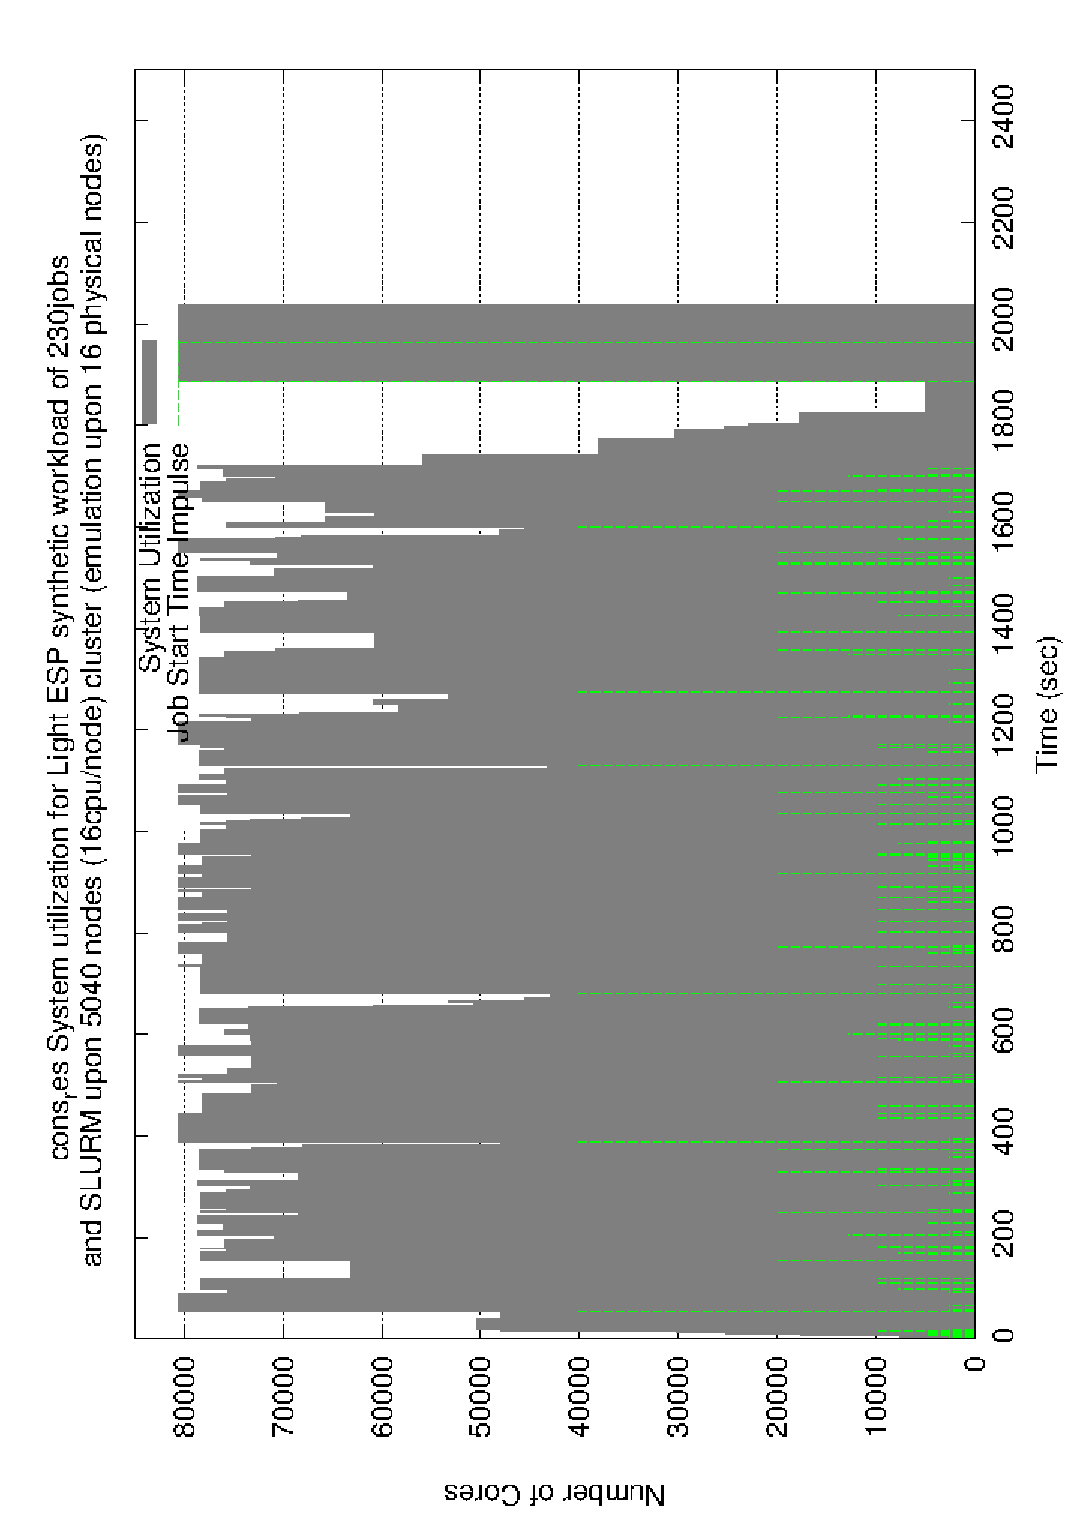
\includegraphics[width=13cm,height=10cm,angle=-90,keepaspectratio]{image/analysis/cons_res_system_util.eps}  
   \end{center}
   \vspace{-1em}
 \caption{system utilization of cores for consumable resource selection plugin for the emulated 5040 nodes HPC system}
   \vspace{-1.5em}
  \label{fig:ConsresSU}
\end{figure}
% End
\subsection{Evaluation of Layouts based Consumable Resource Selection}
System utilization of the HPC system is important property and vary by different scheduler and selector combination. From the system utilization results, we can measure how much resource was used and throughput of the jobs workload to conclude the system level performance. The results of system utilization of the different select plugin follows the same behaviour overall, that is clearly shown in the figure \ref{fig:ConsresSU}, \ref{fig:ConsresLaySU} and \ref{fig:ConsresEeSU}. All the resource selection plugin has the same throughput (i.e. the workload of jobs finish at the same time). Even though the system utilization and throughput is same for overall, the number of jobs waiting time increased. Waiting time is the difference between job submission time and job allocation time. Due to the selection policy or implementation of resource selection plugin, waiting time will be increased. Due to the implementation overhead in cons\_res\_layout plugin, cons\_res\_layout jobs waiting time is higher than cons\_res plugin as shown in the figure \ref{fig:WT-CR-CRL}. In the new cons\_res\_layout policy is not changed, so the implementation is the only reason for the overhead. In the figure\ref{fig:WT-CR-CRL} cumulative distributive function distributes the number of jobs based on the waiting time, the distribution shows the cons\_res plugin has large number of nodes having less waiting time than the cons\_res\_layout plugin. 
\par
The overhead for the job waiting time is due to the resource selection performance, so the time required for the resource selection was calculated in the micro seconds and the results are plotted in the figure \ref{fig:IndPerfCR-CRL}. From the figure \ref{fig:IndPerfCR-CRL}, individual jobs resource selection time was increased twice, so the jobs waiting time was increased in the same rate. In the two experiments of different plugins used ESP benchmark and same program, so the execution time cumulative distributive function will be same.
%, this is clearly shown in the figure \ref{fig:ET-CR-CRL}.  
\vspace{-0.6 cm}
 % Image of LAYOUTS
\begin{figure}[H]%placement
  \centering
   \begin{center}
   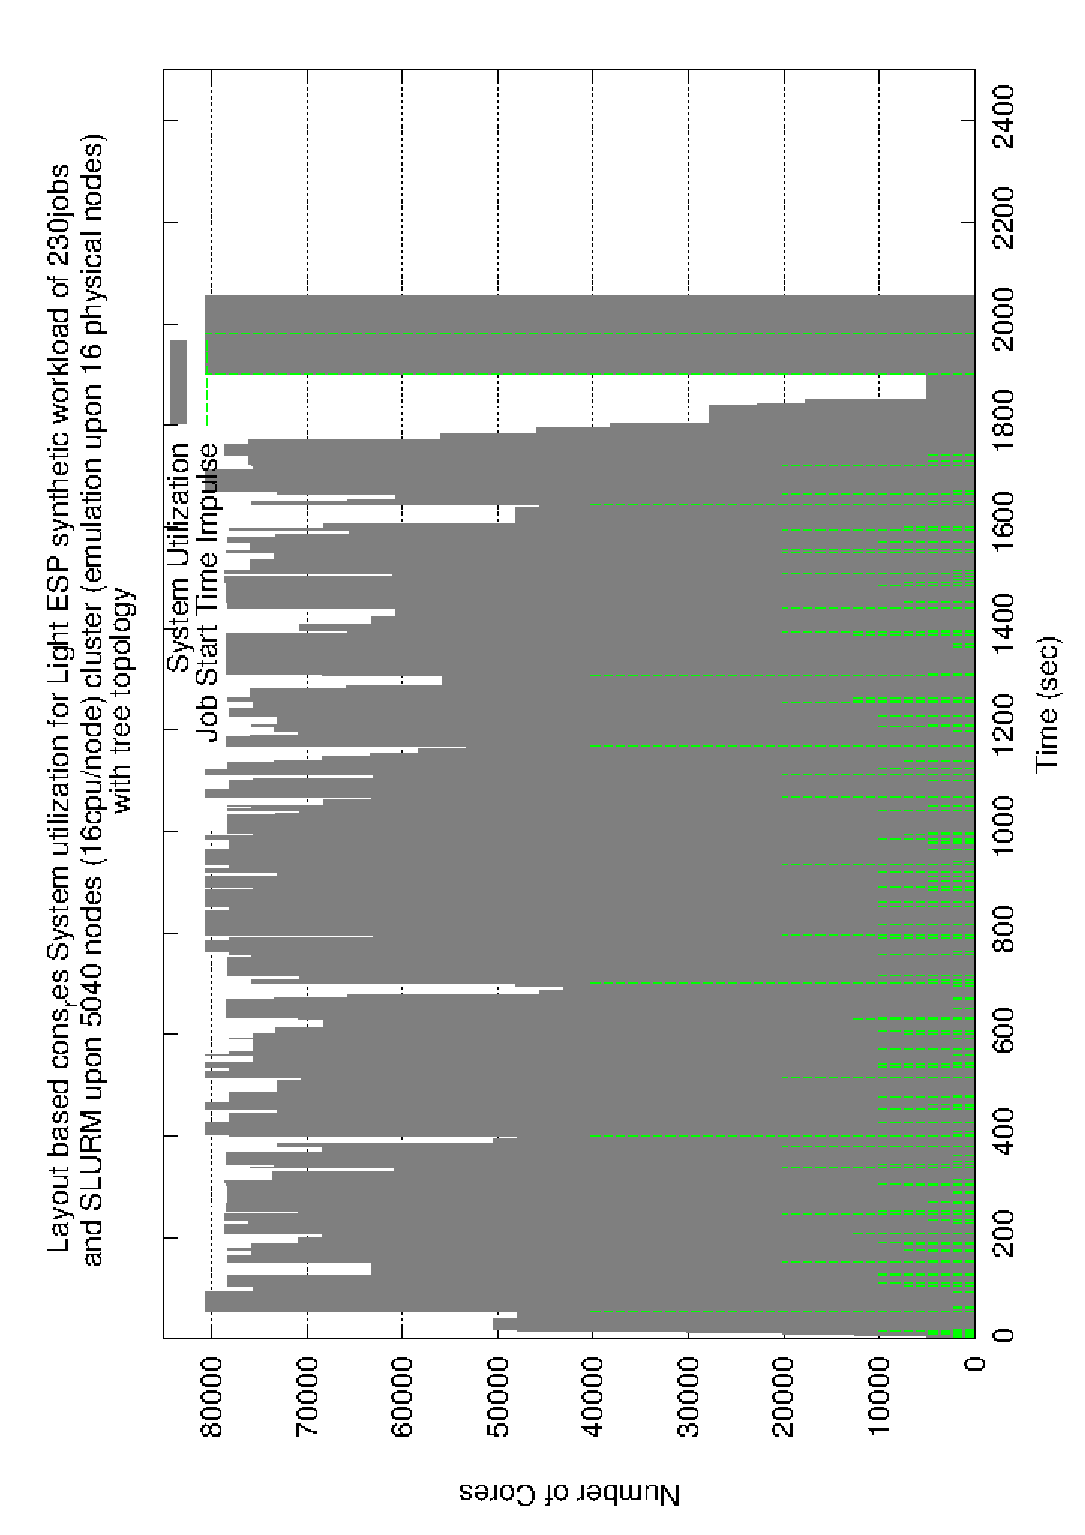
\includegraphics[width=13cm,height=10cm,angle=-90,keepaspectratio]{image/analysis/cons_res_layout_system_util.eps} 
   \end{center}
   \vspace{-1em}
 \caption{System utilization of cores for layouts based consumable resource selection plugin system for the emulated 5040 nodes HPC system}
   \vspace{-0.9em}
  \label{fig:ConsresLaySU}
\end{figure}
% End

 % Image of LAYOUTS
\begin{figure}[H]%placement
  \centering
   \begin{center}
   \includegraphics[width=13cm,height=10cm,angle=-90,keepaspectratio]{image/analysis/CRLP_SU.pdf} 
   \end{center}
   \vspace{-1.5em}
 \caption{System utilization of cores for the energy efficient layouts based resource selection plugin for the emulated 5040 nodes HPC system}
 \vspace{-2cm}
  \label{fig:ConsresEeSU}
\end{figure}

 % Image of LAYOUTS
\begin{figure}[H]%placement
  \centering
   \begin{center}
   \includegraphics[width=13cm,height=10cm,keepaspectratio]{image/analysis/cdf-WT-CR-CRL.pdf} 
   \end{center}
   \vspace{-1em}
 \caption{Cumulative distributive function for the cons\_res and cons\_res\_layout waiting time. Here no\_overhead means without any verbosity the experiment was performed}
 \vspace{-1.5em}
  \label{fig:WT-CR-CRL}
\end{figure}

% % Image of LAYOUTS
%\begin{figure}[H]%placement
%  \centering
%   \begin{center}
%   \includegraphics[width=13cm,height=10cm,keepaspectratio]{image/analysis/cdf-exec-CR-CRL.pdf} 
%   \end{center}
%   \vspace{-1em}
% \caption{Cumulative distributive function for the cons\_res and cons\_res\_layout execution time of 230 jobs.}
% \vspace{-1.5em}
%  \label{fig:ET-CR-CRL}
%\end{figure}
%% End

% Image of LAYOUTS
\begin{figure}[H]%placement
  \centering
   \begin{center}
   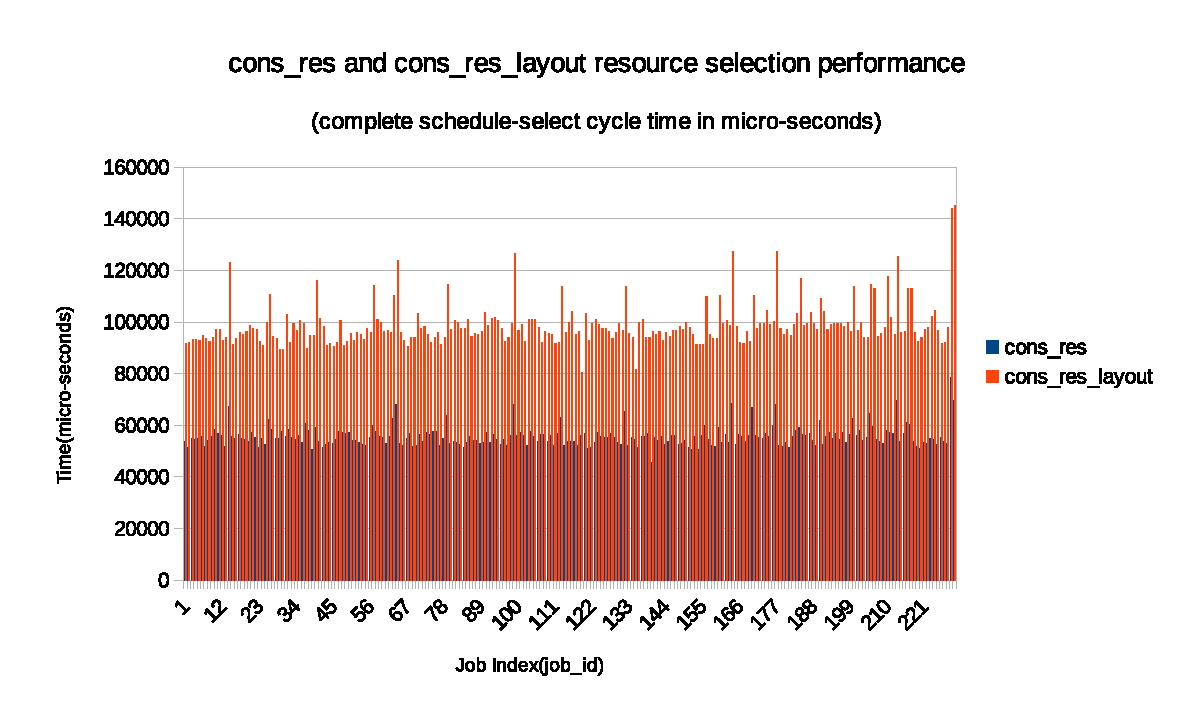
\includegraphics[width=13cm,height=10cm,keepaspectratio]{image/analysis/cr-crl-time-micro.eps} 
   \end{center}
   \vspace{-1em}
 \caption{Individual jobs resource selection time for the cons\_res and cons\_res\_layout plugins for 230 jobs. Cons\_res\_layout plugin individual resource selection performance is increased twice than earlier cons\_res plugin.}
 \vspace{-1.5em}
  \label{fig:IndPerfCR-CRL}
\end{figure}
% End
\subsection{Evaluation of Energy Efficient Consumable Resource Selection}
 The new cons\_res\_layout plugin performance was same as earlier cons\_res plugin performance system wise, but the individual resource selection performance has considerable overhead. Even though the individual resource selection performance was affected, new cons\_res\_layout plugin is flexible to change code. The cons\_res\_layout plugin was enhanced to support energy criteria easily. Energy efficient resource selection policy and layouts plugin used to manage resources  were discussed more detailed in the section 5.2. Best-fit and energy efficient selection policy was used in cons\_res\_power, so the energy consumption will be less than the earlier cons\_res plugin. cons\_res\_power plugin is not the new plugin, it is the enhancement of cons\_res\_layout plugin.
\par
Energy consumed by the cluster is calculated in the frequency of job allocation and cancel to generate the contiguous power consumption. The calculated power consumption was plotted using gnuplot script, the energy consumption of the cons\_res\_power plugin is much better than the cons\_res plugin from the figure \ref{fig:EnergyCR}, \ref{fig:EnergyCRLP} and \ref{fig:EnergyCR-CRLP}. From the experiment results new cons\_res\_power plugin decreased the power consumption by 3.8 \% than old cons\_res plugin. 
\par
Even though the power consumption was decreased by the new energy efficient resource selection policy, individual resource selection performance was decreased three times than earlier cos\_res approach. The new cons\_res\_power plugin used another layout plugin, large number of get operation and large number of set operation of the power value in the node evaluation function. The performance overhead of resource selection was reflected in the waiting time of the jobs. The performance overhead is clearly shown in the figure \ref{fig:IndPerfCR-CRL-CRLP} and \ref{fig:WT-CR-CRL-CRLP}. Resource selection performance is in micro seconds, so the performance overhead does not affect the throughput of the HPC system. New cons\_res\_power increases resource fragmentation within HPC resources, so some jobs will not be satisfied and job waiting time will increase. 
%Cons\_res and cons\_res\_power supporting topology aware resource selection, so the communication will be same. If the communication latency is same then the performance of the application will be same. This is clearly shown in the figure \ref{fig:ET-CR-CRLP}.
  % Image of LAYOUTS
\begin{figure}[H]%placement
  \centering
   \begin{center}
   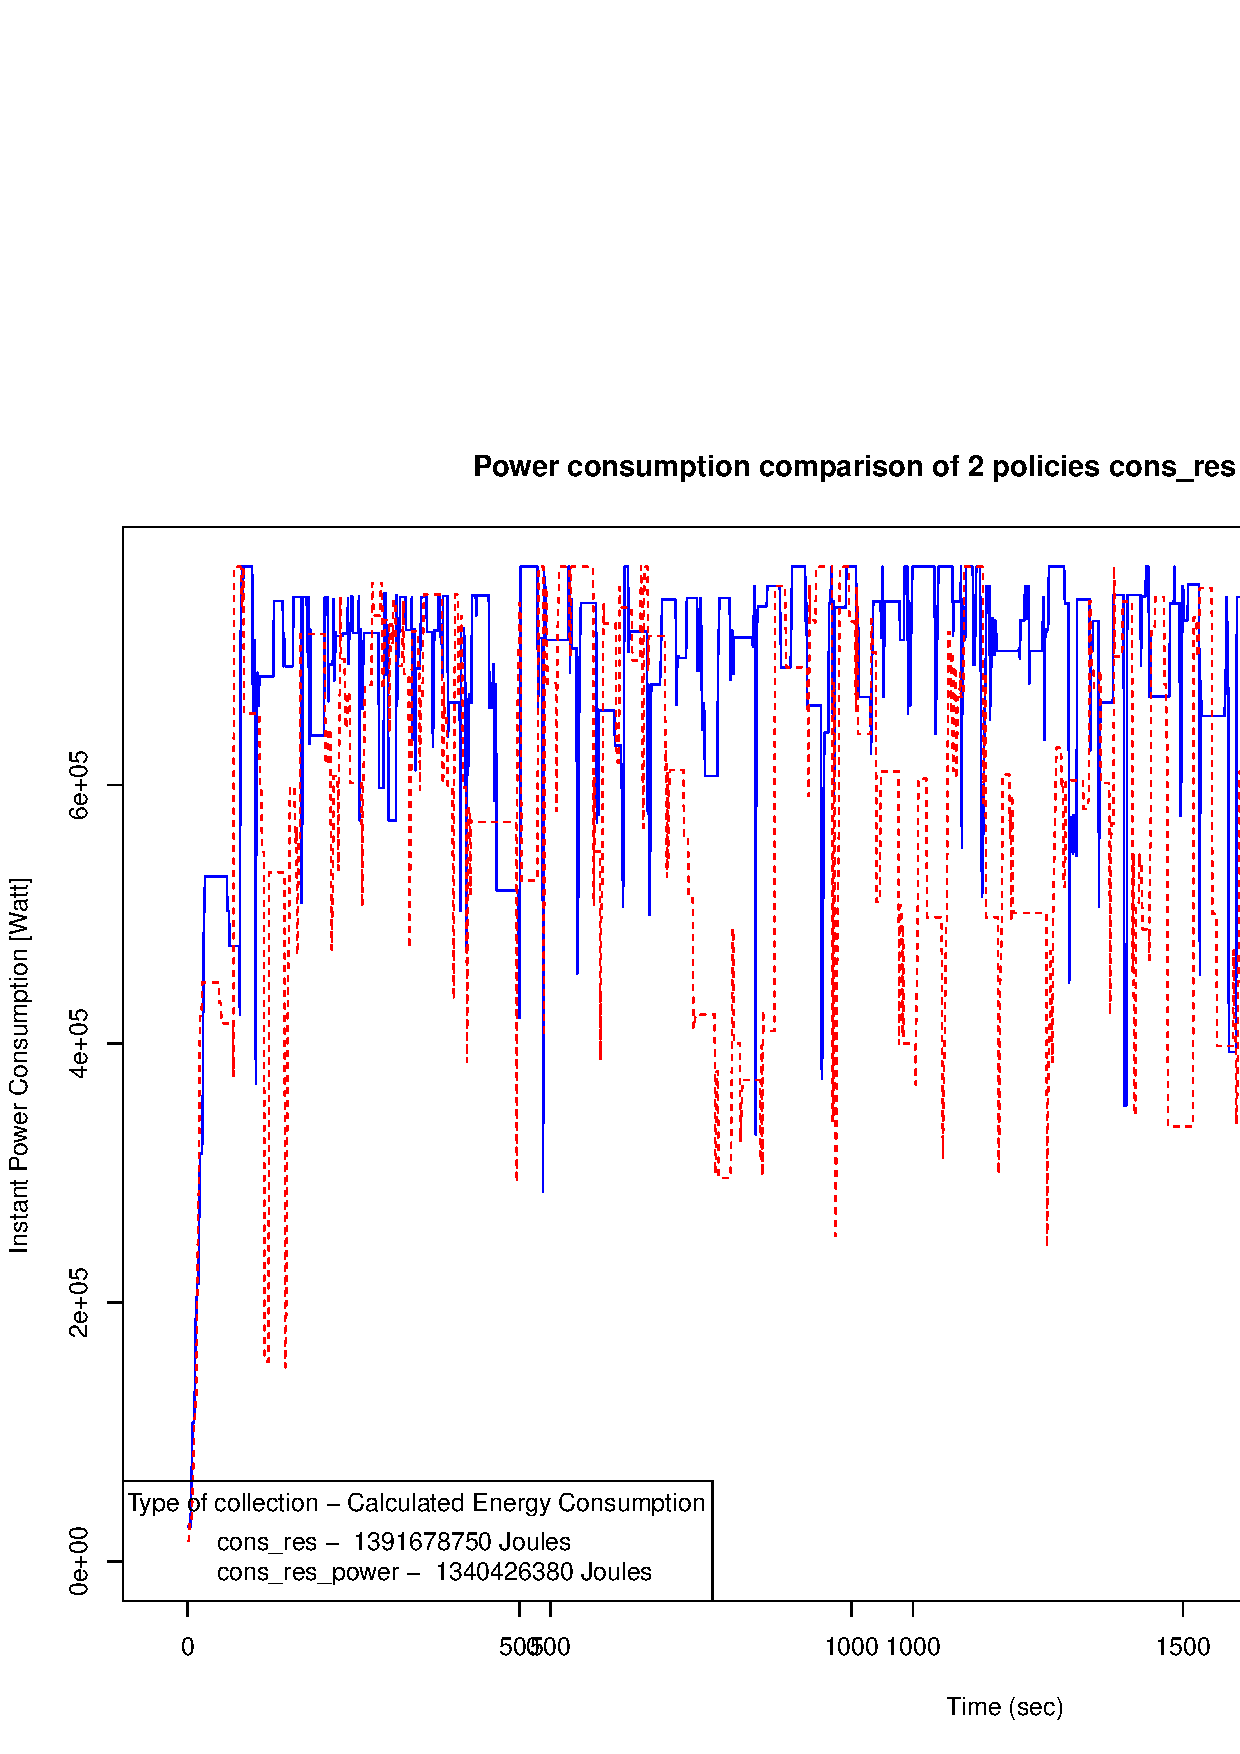
\includegraphics[scale=0.3,keepaspectratio]{image/analysis/cr_crl_31_ju.pdf} 
   \end{center}
   \vspace{-1em}
 \caption{System power utilization comparison for earlier cons\_res plugin and energy efficient cons\_res\_power plugin. Cons\_res\_power decreased overall power consumption by 3.8 percentage than earlier cons\_res plugin.}
 \vspace{-1.5em}
  \label{fig:EnergyCR-CRLP}
\end{figure}
% End
 % Image of LAYOUTS
\begin{figure}[H]%placement
  \centering
   \begin{center}
   \includegraphics[scale=0.3,keepaspectratio] {image/analysis/cr_31_ju.png} 
   \end{center}
   \vspace{-1em}
 \caption{System power utilization for the normal cons\_res plugin}
 \vspace{-1.5em}
  \label{fig:EnergyCR}
\end{figure}
% End

 % Image of LAYOUTS
\begin{figure}[H]%placement
  \centering
   \begin{center}
   \includegraphics[scale=0.3,keepaspectratio]{image/analysis/crl_pl_ju_31.png} 
   \end{center}
   \vspace{-1em}
 \caption{System power utilization for the energy efficient cons\_res\_power plugin}
 \vspace{-1.5em}
  \label{fig:EnergyCRLP}
\end{figure} 
 % Image of LAYOUTS
\begin{figure}[H]%placement
  \centering
   \begin{center}
   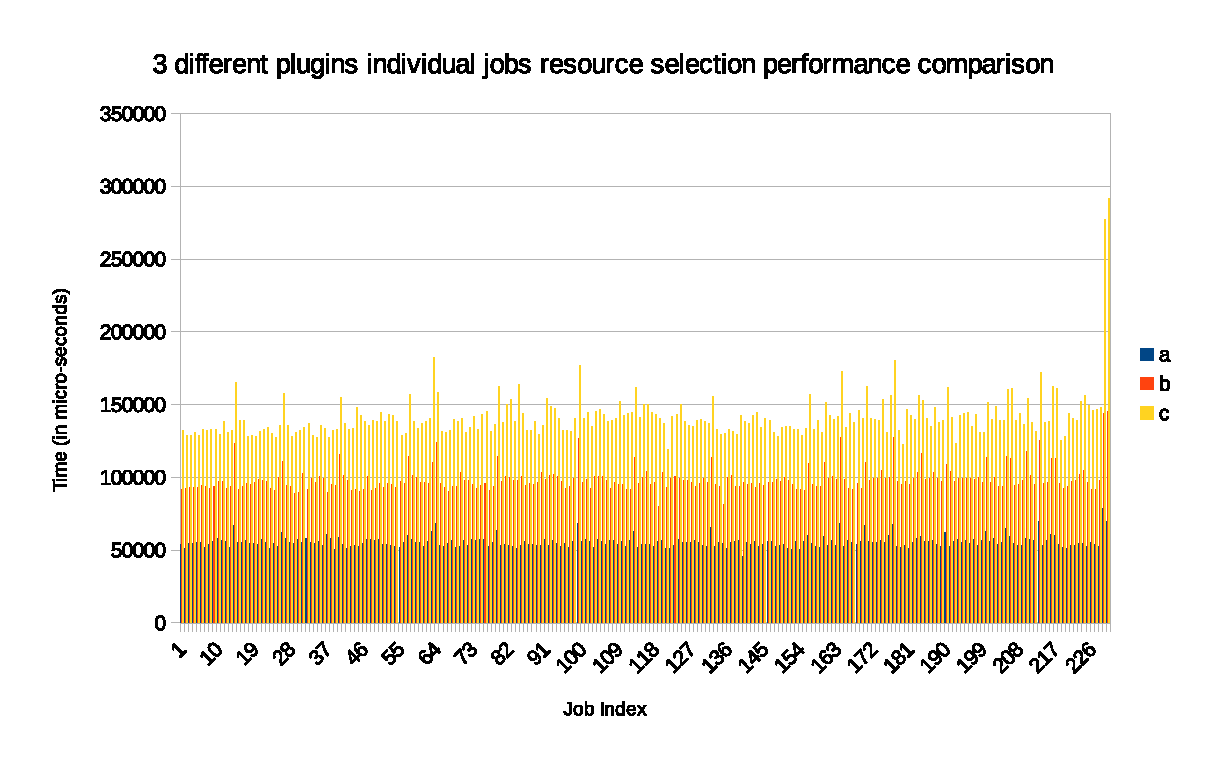
\includegraphics[width=13cm,height=10cm,keepaspectratio]{image/analysis/cr-crl-crlp-time-micro-2.eps} 
   \end{center}
   \vspace{-1em}
 \caption{Individual jobs resource selection time for the cons\_res, cons\_res\_layout and cons\_res\_layout\_power plugins for 230 jobs. In this figure legends \textbf{a} means cons\_res, \textbf{b} means cons\_res\_layout, \textbf{c} means cons\_res\_layout\_power. Cons\_res\_plugin plugin individual resource selection performance is increased thrice than earlier cons\_res plugin.}
 \vspace{-1.5em}
  \label{fig:IndPerfCR-CRL-CRLP}
\end{figure}
% End

 % Image of LAYOUTS
\begin{figure}[H]%placement
  \centering
   \begin{center}
   \includegraphics[width=13cm,height=10cm,keepaspectratio]{image/analysis/cdf-WT-cr-crl-crlp-wt.pdf} 
   \end{center}
   \vspace{-1em}
 \caption{Cumulative distributive function for the cons\_res, cons\_res\_layout and cons\_res\_layout \_power waiting time.}
 \vspace{0.5cm}
  \label{fig:WT-CR-CRL-CRLP}
\end{figure}
%% End
% % Image of LAYOUTS
%\begin{figure}[H]%placement
%  \centering
%   \begin{center}
%   \includegraphics[width=13cm,height=10cm,keepaspectratio]{image/analysis/cdf-exec-SLURM-1024-16384_2.eps} 
%   \end{center}
%   \vspace{-1em}
% \caption{Cumulative distributive function for the cons\_res and cons\_res\_power execution time. Execution time is following the same behaviour, so performance of two plugins are same}
% \vspace{-1.5em}
%  \label{fig:ET-CR-CRLP}
%\end{figure}
%% End
%================== Conclusion ================

\chapter{Conclusion and Future Work}
\vspace{-0.2cm}
\section{Conclusion}
Resource selection is the vital operation like job scheduling in the RJMS. In SLURM consumable resource selection has a lot of features, so throughout the report cons\_res plugin and its enhancement was discussed and implemented. This report explains the new perspective of resource selection implementation, resource management and different criteria based resource selection. SLURM\cite{JetteSLURM} like RJMS plugin enhancement is easier by using the new LAYOUTS\cite{ChevallierLAYOUTS} based resource management. LAYOUTS generic resource management framework has basic APIs and some of them are costly at specific situation, so the new APIs are developed to surpass the performance issuing APIs. 
\par
Consumable resource selection plugin was implemented based on the LAYOUTS framework. New cons\_res\_layout manages resources in the layout plugins and keep policy in the code plugin, this separation enhance the code maintenance. New resource selection plugin(cons\_res\_layout) system utilization and throughput of the workload is same, but the individual jobs resource selection performance was increased twice and the jobs waiting time is increased at the same rate. Select plugin policy or implementation method is the reason for performance overhead of different plugins. Cons\_res\_layout plugin used same topology aware resource selection algorithm in cons\_res, but implementation was based on the LAYOUTS. Cons\_res\_layout plugin using two layout plugin and one plugin entity attributes information is updated from the calculated value of another plugin affects the performance of resource selection. Individual jobs resource selection performance difference is in micro seconds, so it does not affect the overall system properties of system utilization and job throughput.
\par
Energy efficiency is the recent trend to reduce the operating cost of the HPC system. Selecting less power consuming nodes with the application's performance consideration is the good characteristic in the HPC system to satisfy both the criteria of user and server. Even though the performance and energy efficiency is of opposite characteristics, the new multi-parameter resource selection achieved both the criteria. 
\par
The energy consumption of the new multi\_parameter(cons\_res\_power) resource selection was reduced by 3.8 \% compared to the old cons\_res plugin. Due to the overhead of new logic and layouts plugin, the individual jobs resource selection performance was increased thrice and the job waiting time is increased at the same rate. Cons\_res\_power job waiting time is considerably better than powercapping\cite{yiannisPowerCap} approach to limit resource allocation. Due to the power budget of HPC system, powercapping will not allocate available resources until the power budget constraint is satisfied.
%================== Future Work ================

\section{Future Work}
LAYOUTS framework currently supporting tree relations only. If the graph or multi-tree relations supported, then the partition entity will be added in the resource management plugin to mange all the resource entities using LAYOUTS framework. Currently energy efficient policy developed to support static and integer values emulated, but the algorithm to adapt for the current node power consumption based on the energy accounting. 
\par 
Current node power consumption was accounted using RAPL or IPMI technique, this is dicussed in the paper\cite{yiannisENERGY_ACCOUNTING}. The real time value(dynamic) was considered to make decision will need to change the current policy. Decision to follow best-fit energy efficient approach or non-energy efficient will be based on the controller system configuration and job submission option. Instead of following the static configuration decision, can use heuristic algorithm to predict the decisions dynamically. If we achieved the heuristic decision for multiple criteria, then the multi parameter resource selection would be heuristic rather static.
\par 
Currently energy and performance was considered as the criterias to select resources. For the two criterias nine possible permutation(redundant and symmetric combination will be negligible) has to consider for the best resource selection decision. If we include temperature as an another criteria, then the resource selection will be complicated and need to change the policy to support all the criterias. 
\par
In the experiment evaluation instantaneous jobs throughput and instantaneous number of job type allocated will give more details about waiting time of job type  and workload sequence. Different policies fragmented resources information for the specific workload give the more details about percentage of fragmentation to enhance the analysis.

%1. energy efficiency based on the RAPL, IPMI.
%3. Include temperature or convert temperature to energy required.
%4. multi-tree topology
%5. multi criteria is possible.
%6. Resource fragment evaluation

%===============================================================================
\bibliographystyle{plain} % plain-fr si rapport en fran�ais
\bibliography{template-report}

%En fran�ais, il peut �tre une bonne id�e de mettre le r�sum� en 4e de couverture... (� ce moment l�, commenter les abstracts avan la ToC !)
%% 4e de couverture
%\cleardoublepage % Goes to an odd page
%\pagestyle{empty} % no page number
%~\newpage % goes to a new even page
%
%\section*{Abstract} \selectlanguage{english}
%Abstract text
%\medskip
%\selectlanguage{french}
%\section*{R�sum�}
%texte de r�sum�

\appendix

%-------------------------------------------------------------------------
\chapter{SLURM Experiment Configuration}
SLURM system configuration has the complete details about the scheduler and select plugin, slurm controller name, port, logging directory, accounting information, cluster topology type and HPC computing nodes to manage and it is very big, so we described only the important configuration information only. 
\section{SLURM System Configuration}
\begin{verbatim}
DebugFlags=SelectType
PriorityType=priority/multifactor
PriorityDecayHalfLife=0
PriorityCalcPeriod=5

PreemptMode=REQUEUE
PreemptType=preempt/qos

TopologyPlugin=topology/tree
SchedulerType=sched/backfill
SelectType=select/cons_res 
SelectTypeParameters=CR_Core_Memory,CR_CORE_DEFAULT_DIST_BLOCK,
 CR_ONE_TASK_PER_CORE

PartitionName=exclusive Nodes=virtual[0-40] Default=YES
 MaxTime=INFINITE State=UP Priority=10 Shared=EXCLUSIVE
PartitionName=shared Nodes=virtual[0-40] MaxTime=INFINITE State=UP
 Priority=30

NodeName=DEFAULT Sockets=2 CoresPerSocket=2 ThreadsPerCore=8
 RealMemory=384 State=IDLE

NodeName=virtual0 NodeHostName=cuzco12 NodeAddr=mo66 Port=17000
NodeName=virtual1 NodeHostName=cuzco12 NodeAddr=mo66 Port=17001
\end{verbatim}
\section{SLURM Topology Configuration}
\begin{verbatim}
SwitchName=switch0 Switches=switch[1-2]
SwitchName=switch1 Switches=switch[3-4]
SwitchName=switch2 Switches=switch[5-6]
SwitchName=switch3 Nodes=virtual[0-1999]
SwitchName=switch4 Nodes=virtual[2000-2999]
SwitchName=switch5 Nodes=virtual[3000-3999]
SwitchName=switch6 Nodes=virtual[4000-5039]
\end{verbatim}
%-------------------------------------------------------------------------
\chapter{Layouts plugin Keys and Key relations}
In SLURM following aggregate functions key relations are defined.
\begin{itemize}
\item Child aggregate functions - Specific operations performed on the children key value and update the calculated value in the parent$'$s key\\ \vspace{0.01em} 
	\begin{enumerate}
		\item KEYSPEC\_UPDATE\_CHILDREN\_SUM   
		\item KEYSPEC\_UPDATE\_CHILDREN\_AVG   
		\item KEYSPEC\_UPDATE\_CHILDREN\_MIN   
		\item KEYSPEC\_UPDATE\_CHILDREN\_MAX   
		\item KEYSPEC\_UPDATE\_CHILDREN\_COUNT 
		\item KEYSPEC\_UPDATE\_CHILDREN\_MASK  
	\end{enumerate}
\item Parent aggregate functions - Specific operations performed on the parents key value and update the calculated value in the child$'$s key\\
	\begin{enumerate}
		\item KEYSPEC\_UPDATE\_PARENTS\_SUM    
		\item KEYSPEC\_UPDATE\_PARENTS\_AVG    
		\item KEYSPEC\_UPDATE\_PARENTS\_MIN    
		\item KEYSPEC\_UPDATE\_PARENTS\_MAX    
		\item KEYSPEC\_UPDATE\_PARENTS\_FSHARE 
		\item KEYSPEC\_UPDATE\_PARENTS\_MASK   
	\end{enumerate}
\end{itemize} 

\section{Node Architecture (cons\_res\_partition) Keys}
\begin{verbatim}
const layouts_keyspec_t keyspec[] = {
{"AllocatedNodeCount",L_T_UINT32,KEYSPEC_UPDATE_CHILDREN_AVG,
"AllocatedSocketCount"}, 
	{"AllocatedSocketCount",L_T_UINT32},
	{"AllocatedCoreCount",L_T_UINT32},
	{"AllocatedThreadsPerCore",L_T_UINT32},
	{"nodecount",L_T_UINT32},  
	{"socketcount",L_T_UINT32}, 
	{"corecount",L_T_UINT32}, 
	{"ThreadsPerCore",L_T_UINT32},  
	{"NumSumNodes", L_T_UINT32, KEYSPEC_UPDATE_CHILDREN_SUM,
	 "nodecount"},  // It is in Cluster
	{"NumSumCoresInCluster",L_T_UINT32, KEYSPEC_UPDATE_CHILDREN_SUM,
	 "NumSumCoresInNode"},
	{"NumSumThreadsInCluster",L_T_UINT32, KEYSPEC_UPDATE_CHILDREN_SUM,
	 "NumSumThreadsInNode"},
	{"NumSumSocketsInCluster",L_T_UINT32, KEYSPEC_UPDATE_CHILDREN_SUM,
	 "NumSumSockets"},
		 // It is in Node
	{"NumSumSockets",L_T_UINT32, KEYSPEC_UPDATE_CHILDREN_SUM,
	 "socketcount"},
	{"NumSumCoresInNode",L_T_UINT32, KEYSPEC_UPDATE_CHILDREN_SUM,
	 "NumSumCores"},
	{"NumSumThreadsInNode",L_T_UINT32, KEYSPEC_UPDATE_CHILDREN_SUM,
	 "NumSumThreads"},	
	{"NumSumCores",L_T_UINT32, KEYSPEC_UPDATE_CHILDREN_SUM,	
	 "corecount"}, //It is in Socket
	{"NumSumThreads",L_T_UINT32, KEYSPEC_UPDATE_CHILDREN_SUM,
	 "ThreadsPerCore"},
	{"AllocatedSumNodes", L_T_UINT32, KEYSPEC_UPDATE_CHILDREN_SUM,
	 "AllocatedNodeCount"},  // It is in Cluster
	{"AllocatedSumCoresInCluster",L_T_UINT32, KEYSPEC_UPDATE_CHILDREN_SUM,
	 "AllocatedSumCoresInNode"},
	{"AllocatedSumSocketsInCluster",L_T_UINT32 ,KEYSPEC_UPDATE_CHILDREN_SUM
	 ,"AllocatedSumSockets"},
	{"AllocatedSumThreadsInCluster",L_T_UINT32, KEYSPEC_UPDATE_CHILDREN_SUM,
	 "AllocatedSumThreadsInNode"},	
	{"AllocatedSumSockets",L_T_UINT32, KEYSPEC_UPDATE_CHILDREN_SUM
	,"AllocatedSocketCount"}, // It is in Node
	{"AllocatedSumCoresInNode",L_T_UINT32, KEYSPEC_UPDATE_CHILDREN_SUM,
	 "AllocatedSumCores"},
	{"AllocatedSumThreadsInNode",L_T_UINT32, KEYSPEC_UPDATE_CHILDREN_SUM,
	 "AllocatedSumThreads"},	
	{"AllocatedSumCores",L_T_UINT32, KEYSPEC_UPDATE_CHILDREN_SUM,
	 "AllocatedCoreCount"}, //It is in Socket
	{"AllocatedSumThreads",L_T_UINT32, KEYSPEC_UPDATE_CHILDREN_SUM,
	 "AllocatedThreadsPerCore"},
	{"Job",L_T_UINT32}, //It indicates which core has which job	
	{NULL}
};
\end{verbatim}
\section{Cluster Topology (cons\_res\_topology) Keys}
\begin{verbatim}
const layouts_keyspec_t keyspec[] = {
	/* base keys */	
	// topology based Node config
	{"AvailableNodeCount",L_T_UINT32}, 
	{"AvailableCpusCount",L_T_UINT16},
	/* Parents aggregated keys */
	// topology based switch configuration
	{"AvailableSumNodesInLevel0", L_T_UINT32, KEYSPEC_UPDATE_CHILDREN_SUM,
	 "AvailableNodeCount"},
	{"AvailableSumCpusInLevel0",L_T_UINT16, KEYSPEC_UPDATE_CHILDREN_SUM,
	 "AvailableCpusCount"},
	{"AvailableSumNodesInLevel1", L_T_UINT32, KEYSPEC_UPDATE_CHILDREN_SUM,
	 "AvailableSumNodesInLevel0"}, 
	{"AvailableSumCpusInLevel1",L_T_UINT16, KEYSPEC_UPDATE_CHILDREN_SUM,
	 "AvailableSumCpusInLevel0"},
	{"AvailableSumNodesInLevel2", L_T_UINT32, KEYSPEC_UPDATE_CHILDREN_SUM,
	 "AvailableSumNodesInLevel1"},
	{"AvailableSumCpusInLevel2",L_T_UINT16, KEYSPEC_UPDATE_CHILDREN_SUM,
	 "AvailableSumCpusInLevel1"},
	{"AvailableSumNodesInLevel3", L_T_UINT32, KEYSPEC_UPDATE_CHILDREN_SUM,
	 "AvailableSumNodesInLevel2"},
	{"AvailableSumCpusInLevel3",L_T_UINT16, KEYSPEC_UPDATE_CHILDREN_SUM,
	 "AvailableSumCpusInLevel2"},
	{NULL}
};
\end{verbatim}
\section{Energy Layout (topology\_power) keys}
\begin{verbatim}
const layouts_keyspec_t keyspec[] = {
        /* base keys */
        // topology based Node config
        {"IdleWatts",L_T_UINT32},
        {"MaxWatts",L_T_UINT32},

        /* Parents aggregated keys */
        // topology based configuration
        {"IdleSumWattsInLevel0", L_T_UINT32,
         KEYSPEC_UPDATE_CHILDREN_SUM, "IdleWatts"},
        {"MaxSumWattsInLevel0",L_T_UINT32,
         KEYSPEC_UPDATE_CHILDREN_SUM, "MaxWatts"},

        {"IdleSumWattsInLevel1", L_T_UINT32,
         KEYSPEC_UPDATE_CHILDREN_SUM, "IdleSumWattsInLevel0"},
        {"MaxSumWattsInLevel1",L_T_UINT32,
         KEYSPEC_UPDATE_CHILDREN_SUM, "MaxSumWattsInLevel0"},

        {"IdleSumWattsInLevel2", L_T_UINT32,
         KEYSPEC_UPDATE_CHILDREN_SUM, "IdleSumWattsInLevel1"},
        {"MaxSumWattsInLevel2",L_T_UINT32,
         KEYSPEC_UPDATE_CHILDREN_SUM, "MaxSumWattsInLevel1"},

        {"IdleSumWattsInLevel3", L_T_UINT32,
         KEYSPEC_UPDATE_CHILDREN_SUM, "IdleSumWattsInLevel2"},
        {"MaxSumWattsInLevel3",L_T_UINT32,
         KEYSPEC_UPDATE_CHILDREN_SUM, "MaxSumWattsInLevel2"},

        {NULL}
};
\end{verbatim}
%-------------------------------------------------------------------------
\chapter{Layouts Configuration File}
All the experiments were done on 5040 nodes configuration and the configuration files are very big, so the following section has the part of configuration file to describe the complete details.
\section{Node Architecture (cons\_res\_partition) Configuration}
\begin{verbatim}
Priority=10
Root=Cluster

#Root or Cluster level Layout configuration
Entity=Cluster Type=Center NumSumNodes=0 NumSumCoresInCluster=0
 NumSumSocketsInCluster=0 AllocatedSumNodes=0 
 AllocatedSumCoresInCluster=0 AllocatedSumSocketsInCluster=0
 AllocatedSumThreadsInCluster=0 NumSumThreadsInCluster=0
 Enclosed=virtual[0-5039]

# Compute node layout configuration 
Entity=virtual0 type=Node nodecount=1 AllocatedNodeCount=0
 NumSumSockets=0 NumSumCoresInNode=0 AllocatedSumSockets=0
 AllocatedSumCoresInNode=0 AllocatedSumThreadsInNode=0 
 NumSumThreadsInNode=0 Enclosed=socket[0-1]
Entity=virtual1 type=Node nodecount=1 AllocatedNodeCount=0
 NumSumSockets=0 NumSumCoresInNode=0 AllocatedSumSockets=0
 AllocatedSumCoresInNode=0 AllocatedSumThreadsInNode=0 
 NumSumThreadsInNode=0 Enclosed=socket[2-3]
 	
#Socket Level layout configuration following
Entity=socket0 type=Socket socketcount=1 NumSumCores=0 
AllocatedSumCores=0 AllocatedSocketCount=0 
AllocatedSumThreads=0 NumSumThreads=0 Enclosed=core[0-7]

#Core level Layout configuration following
Entity=core[0-80639] type=Core ThreadsPerCore=1 
AllocatedThreadsPerCore=0 AllocatedCoreCount=0 corecount=1
\end{verbatim}
\section{Cluster Topology (cons\_res\_topology) Configuration}

\begin{verbatim}
Priority=10
Root=switch0

#Root or Cluster level Layout configuration
#switch or tree topolgy configuration
Entity=switch0 Type=Switch AvailableSumNodesInLevel2=0
 AvailableSumCpusInLevel2=0 Enclosed=switch[1-2]

Entity=switch1 Type=Switch AvailableSumNodesInLevel1=0 
 AvailableSumCpusInLevel1=0 Enclosed=switch[3-4]
Entity=switch2 Type=Switch AvailableSumNodesInLevel1=0 
 AvailableSumCpusInLevel1=0 Enclosed=switch[5-6]
Entity=switch3 Type=Switch AvailableSumNodesInLevel0=0
 AvailableSumCpusInLevel0=0  Enclosed=virtual[0-1999]
Entity=switch4 Type=Switch AvailableSumNodesInLevel0=0 
 AvailableSumCpusInLevel0=0 Enclosed=virtual[2000-2999]
Entity=switch5 Type=Switch AvailableSumNodesInLevel0=0
 AvailableSumCpusInLevel0=0 Enclosed=virtual[3000-3999]
Entity=switch6 Type=Switch AvailableSumNodesInLevel0=0
 AvailableSumCpusInLevel0=0 Enclosed=virtual[4000-5039]
# Compute node layout configuration 
Entity=virtual[0-5039] type=Node AvailableNodeCount=0
 AvailableCpusCount=0
\end{verbatim}

\section{Energy Layout (topology\_power) Configuration}

\begin{verbatim}
Priority=10
Root=switch0
#Root or Cluster level Layout configuration
#switch or tree topolgy configuration
Entity=switch0 Type=Switch IdleSumWattsInLevel2=0 MaxSumWattsInLevel2=0
 Enclosed=switch[1-2]
Entity=switch1 Type=Switch IdleSumWattsInLevel1=0 MaxSumWattsInLevel1=0
 Enclosed=switch[3-4]
Entity=switch2 Type=Switch IdleSumWattsInLevel1=0 MaxSumWattsInLevel1=0
 Enclosed=switch[5-6]
Entity=switch3 Type=Switch IdleSumWattsInLevel0=0 MaxSumWattsInLevel0=0
 Enclosed=virtual[0-1999]
Entity=switch4 Type=Switch IdleSumWattsInLevel0=0 MaxSumWattsInLevel0=0
 Enclosed=virtual[2000-2999]
Entity=switch5 Type=Switch IdleSumWattsInLevel0=0 MaxSumWattsInLevel0=0
 Enclosed=virtual[3000-3999]
Entity=switch6 Type=Switch IdleSumWattsInLevel0=0 MaxSumWattsInLevel0=0
 Enclosed=virtual[4000-5039]
# Compute node layout configuration 
Entity=virtual[0-1999] type=Node IdleWatts=120 MaxWatts=170
Entity=virtual[2000-2999] type=Node IdleWatts=110 MaxWatts=160
Entity=virtual[3000-3999] type=Node IdleWatts=130 MaxWatts=180
Entity=virtual[4000-5039] type=Node IdleWatts=50 MaxWatts=100
\end{verbatim}
%-------------------------------------------------------------------------
\chapter{Resource selection implementation in Select plugins}
\vspace{-1.2cm}
% Image of LAYOUTS
\begin{figure}[H]%placement
  \centering
   \begin{center}
   \includegraphics[scale=0.5,keepaspectratio]{image/resource-selection-sequence.png} 
   \end{center}
   \vspace{-1em}
 \caption{Actual resource selection algorithm starts from the function select\_nodes. The function flow and naming convention is same for cons\_res and cons\_res\_layout select plugin. In the sequence diagram function select\_nodes\_ctd is the continuation of select\_node function. Eval\_nodes function is the heart of resource selection to support topology\_aware and multi-parameters. Cons\_res and Cons\_res\_layout plugin used the same function flow and function naming.}
 \vspace{-0.5cm}
  \label{fig:a-job-rs}
\end{figure}
% End
 % Image of LAYOUTS
\begin{figure}[H]%placement
  \centering
   \begin{center}
   \includegraphics[scale=0.5,keepaspectratio]{image/resource-selection-sequence-1.png} 
   \end{center}
   \vspace{-1em}
 \caption{High level function flow to satisfy jobs constraint and job details gathering. select\_g\_job\_test is the resource selection mechanism function call and it wraps the specific plugin function call of select\_p\_job\_test. Cons\_res and Cons\_res\_layout plugin used the same function flow and function naming.}
 \vspace{0.5cm}
  \label{fig:a-job-constraint}
\end{figure}
% End

 

%-------------------------------------------------------------------------

\end{document}
